%%%%%%%%%%%%%%%%%%%%%%%%%%%%%%%%%%%%%%%%%%%%%%%%%%%%%%%%%%%%
%%%%%%%%%%%%%%%%%%%%%%%%%%%%%%%%%%%%%%%%%%%%%%%%%%%%%%%%%%%%
%\section{A proposição e a anotação}

Como ponto de partida,
é definida uma proposição como sendo a variável manipulada em seu valor máximo.
Como o sistema proposto neste trabalho tem um controle de motor de corrente contínua,
sendo a tensão média aplicada ao motor, para controle da sua velocidade,
através de um acionamento do tipo modulação por largura de pulso (\emph{PWM}),
cujo parâmetro é o \emph{duty cycle}, ou seja, o percentual em que o nível lógico
da modulação está atuando,
assim, quando a variável manipulada for máxima,
significa que a proposição alcançou a verdade.
Pode-se então definir a proposição como sendo:
"P: O acionamento do motor está ajustado para velocidade máxima."

A velocidade de rotação do motor é a variável controlada,
e a sua relação com a variável manipulada se dá pela relação direta
no processo de calibração do controlador,
em que a velocidade máxima do sistema é definida como ponto de verdade do reticulado.
Assim, o controlador opera como um sistema em malha aberta,
ajustando a variável manipulada para o máximo,
deve-se obter o máximo da variável controlada,
definindo assim o ponto de verdade do reticulado.
De forma análoga, ajustando a variável manipulada para o mínimo,
normalmente zero, deve-se obter o mínimo da variável controlada,
velocidade zero, ponto de falsidade do reticulado.

Como os pontos de verdade e falsidade definem os respectivos de
máxima e mínima da variável controlada, velocidade de rotação do motor,
toda extensão de velocidades está contida sobre a reta perfeitamente definida,
assim a reta do grau de certeza contém todas as possibilidades de velocidade,
dado um erro zero entre valor desejado, valor de referência ou \emph{set point},
e o valor lido pelo sensor de velocidade, variável controlada.

O valor desejado então é representado pelo grau de evidência favorável ($\mu$),
enquanto que o complemento do valor do sensor é o grau de evidência contrário ($\lambda$).
Como o $\lambda$ é o complemento do sensor,
pode-se assumir o sensor como um segundo segundo grau de evidência favorável.
Assim adota-se $\mu_0 = \mu$ e $\mu_1 = (1 - \lambda)$.



O diagrama da Figura \ref{fig:diagramaBlocosLPAEt} apresenta 
a planta do sistema $g(t)$ tendo como saída a 
variável controlada $c(t)$, 
que é a velocidade de rotação do disco 
acoplado ao eixo do motor, 
e como entrada a variável manipulada $u(t)$, 
que é o parâmetro do \emph{PWM} 
que produz a sinal aplicado à planta.



\begin{figure}[!h]%%%%%%%%%%%%%%%%%%%%%%%%%%%%%%%%fg
\centering
\caption{Diagrama de blocos do controle utilizando a LPA$E\tau$}
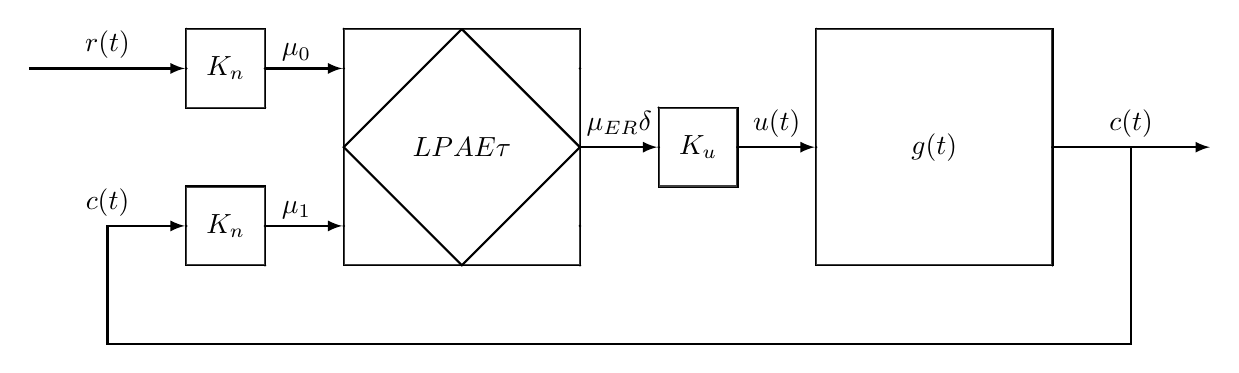
\begin{tikzpicture}[scale=1.0]
\tikzset{ >=latex, inner sep=0pt, outer sep=0pt,  }

%\draw [lightgray, dashed](0,0) grid (15,4.2);

%%% Blocos 

% Kn normalização rps -> 0..1
\node [fill=black, circle] (KSP0) at (2.0,4.0) { };
\node [fill=black, circle] (KSP1) at (3.0,3.0) { };
\draw[thick] (KSP0) rectangle (KSP1);
\fill[white, nearly transparent] (KSP0) rectangle (KSP1);
\node [fill=black, circle] (KSPin)  at (2.0,3.5) { }; 
\node [fill=black, circle] (KSPout) at (3.0,3.5) { }; 
\node (Kn1) at (2.5,3.5) {$K_n$};

% Kn Sensor
\node [fill=black, circle] (KS0) at (2.0,2.0) { };
\node [fill=black, circle] (KS1) at (3.0,1.0) { };
\draw[thick] (KS0) rectangle (KS1);
\fill[white, nearly transparent] (KS0) rectangle (KS1);
\node [fill=black, circle] (KSin)  at (2.0,1.5) { };
\node [fill=black, circle] (KSout) at (3.0,1.5) { };
\node (Kn2) at (2.5,1.5) {$K_n$};

% LPAEt
\node [fill=black, circle] (LPA0) at (4,4.0) { };
\node [fill=black, circle] (LPA1) at (7,1.0) { };
\draw[thick] (LPA0) rectangle (LPA1);
\fill[white, nearly transparent] (LPA0) rectangle (LPA1);
\draw [thick] (5.5,4.0) -- (7.0,2.5) -- (5.5,1.0) -- (4.0,2.5) -- (5.5,4.0);
\node (LPA2v) at (5.5,2.5) {$LPAE\tau$};
\node [fill=black, circle] (LPAu0)  at (4.0,3.5) { };
\node [fill=black, circle] (LPAu1)  at (4.0,1.5) { };
\node [fill=black, circle] (LPAgc)  at (7.0,3.5) { };
\node [fill=black, circle] (LPAs)   at (7.0,2.5) { };
\node [fill=black, circle] (LPAgct) at (7.0,1.5) { };
\node (LPA2vu0)  at (3.4,3.7) {$\mu _0$};
\node (LPA2vu1)  at (3.4,1.7) {$\mu _1$};

% Kn u(t)
\node [fill=black, circle] (KU0) at (8.0,3.0) { };
\node [fill=black, circle] (KU1) at (9.0,2.0) { };
\draw[thick] (KU0) rectangle (KU1);
\fill[white, nearly transparent] (KU0) rectangle (KU1);
\node [fill=black, circle] (KUin)  at (8.0,2.5) { };
\node [fill=black, circle] (KUout) at (9.0,2.5) { };
\node (Ku2) at (8.5,2.5) {$K_u$};


% Planta
\node [fill=black, circle] (GT0) at (10,4.0) { };
\node [fill=black, circle] (GT1) at (13,1.0) { };
\draw[thick] (GT0) rectangle (GT1);
\fill[white, nearly transparent] (GT0) rectangle (GT1);
\node [fill=black, circle] (GTin)  at (10.0,2.5) { };
\node [fill=black, circle] (GTout) at (13.0,2.5) { };
\node (planta) at (11.5,2.5) {$g(t)$};



%%% Linhas 

% set point
\draw [->, thick] (0.0,3.5) -- (KSPin);
\node (rt) at (1.0,3.8) {$r(t)$};

% GT -> fim
\draw [->, thick] (GTout) -- (15,2.5);
\node (ct) at (14.0,2.8) {$c(t)$};
\node (ct) at (1.0,1.8) {$c(t)$};

% normalização 0..1 -> LPA2v u0
\draw [->, thick] (KSPout) -- (LPAu0);

% normalização 0..1 -> LPA2v u1
\draw [->, thick] (KSout) -- (LPAu1);

% LPAEt -> Ku
\draw [->, thick] (LPAs) -- (KUin);
\node (ut) at (7.5,2.8) {$\mu_{ER}\delta$};

% Ku -> GT
\draw [->, thick] (KUout) -- (GTin);
\node (ut) at (9.5,2.8) {$u(t)$};

% GT -> Kn Sensor
\draw [->, thick] (GTout) -- (14.0,2.5) -- (14.0,0.0) -- (1.0,0.0) -- (1.0,1.5) -- (KSin);


\end{tikzpicture}
\label{fig:diagramaBlocosLPAEt}

{\vspace{0.2cm} \small Fonte: Próprio autor}
\end{figure}
%%%%%%%%%%%%%%%%%%%%%%%%%%%%%%%%%%%%%%%%



A variável manipulada $u(t)$ é produzida pelo 
bloco controlador $LPAE\tau$, 
e este recebe seus parâmetros no formato dos 
graus de evidência favoráveis $\mu_0$ e $\mu_1$.
Sendo o parâmetro $\mu_1$ 
convertido internamente em $\lambda$ 
como grau de evidência contrária.

Os dois parâmetros que vão gerar os graus de evidência 
possuem a mesma natureza, a mesma escala, 
são a velocidade desejada e a velocidade lida pelo sensor,
de modo a poder comparar e utilizá-las nas operações da
LPA$E\tau$. 
Para adequação da escala das grandezas 
de referência $r(t)$ e da variável controlada $c(t)$
ao intervalo de trabalho dos parâmetros da LPA$E\tau$, 
é inserido um bloco de normalização do sinal em cada entrada,
bem como na saída.


Para a normalização os blocos $K_n$ realizam as seguinte operações:

\begin{equation}%%%%%%%%%%%%%%%%%%%%%%%%%%%%%%%%%% eq
\mu_0 = \frac{ r(t)}{c(t)_{\text{máx}}} \ \ \ \ \ \ \ \ \mu_1 = \frac{c(t)}{c(t)_{\text{máx}}}
\label{eq:nomaliza}
\end{equation}%%%%%%%%%%%%%%%%%%%%%%%%%%%%%%%%%%%%
\vspace{-0.4cm}
onde:

$c(t)_{\text{máx}}$: é a velocidade máxima produzida pelo sistema.


Para a normalização do bloco $K_u$ é realizada a seguinte operação:

\begin{equation}
u(t) = \mu_{ER}\delta . 100
\end{equation}

\vspace{-0.4cm}
onde:

$\mu_{ER}\delta$: valor contido no intervalo fechado [0, 1].

$u(t)$: valor contido no intervalo [0, 100] 
referente ao parâmetro(\%) do acionamento PWM.




%%%%%%%%%%%%%%%%%%%%%%%%%%%%%%%%%%%%%%%%%%%%%%%%%%%%%%%%%%%%
%%%%%%%%%%%%%%%%%%%%%%%%%%%%%%%%%%%%%%%%%%%%%%%%%%%%%%%%%%%%
%\newpage

Tendo o $\mu_1 (\mu)$ e o $\mu_1 (1-\lambda)$ ajustados dessa forma,
tem-se que todas as possibilidades consideráveis estão contidas dentro do reticulado,
e a sua divisão em regiões é mandatória para a realização do controle e o tratamento de
falhas, mas que seus limiares vão depender intrinsecamente do sistema controlado.

As regiões aqui definidas para a realização do controle proposto
são expostas de forma incremental e complementar no reticulado,
definindo o controlador aqui proposto,
bem como as nomenclaturas para tal aplicação,
diferentes das implementações em trabalhos anteriores,
por ser uma abordagem diferenciada destes.


\section{Região de incerteza positiva e negativa}

A região de incerteza está contemplada em toda a região diferente da
reta perfeitamente definida, local em que o Grau de Incerteza vale zero,
tendo acima desta a denominação de região de incerteza positiva
enquanto que abaixo a denominação é região de incerteza negativa,
denominações que serão utilizados no reticulado para a aplicação
apresentada neste trabalho.


%%%%%%%%%%%%%%%%%%%%%%%%%%%%%%%%%%%%%%%%%%%%%%%%%%%%%%%%% Fg
\begin{figure}[!h]%%%%%%%%%%%%%%%%%%%%%%%%%%%%%%%%%%%%%%%%%%
\centering
\caption{Representação das regiões de incerteza não nulas (positiva e negativa)}
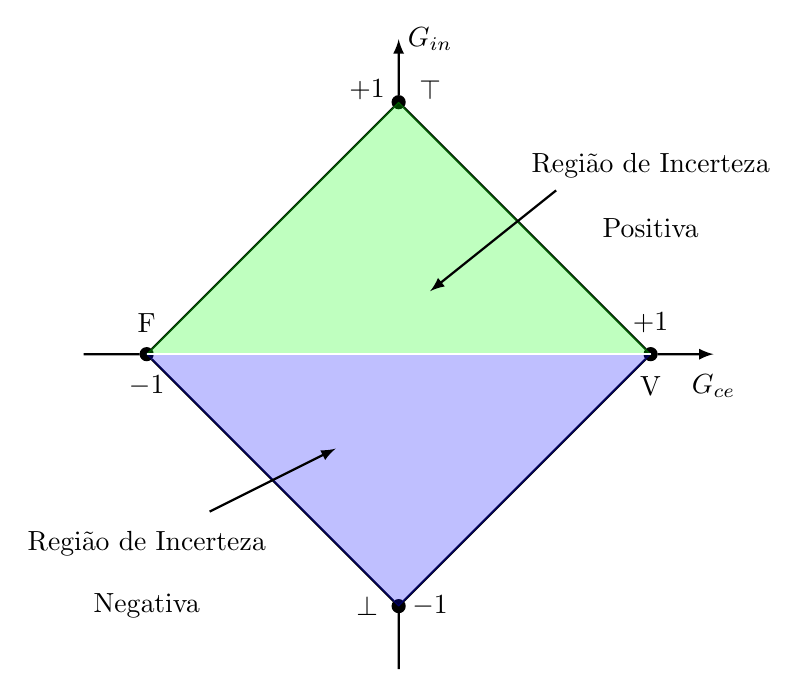
\begin{tikzpicture}[scale=0.80]
\tikzset{ >=latex, inner sep=0pt, outer sep=0pt,  }

%\draw [lightgray, dashed](0,0) grid (10,10);

\node [fill=black, circle] (V) at (9,5) {:};
\node [fill=black, circle] (F) at (1,5) {:};
\node [fill=black, circle] (T) at (5,9) {:};
\node [fill=black, circle] (L) at (5,1) {:};

\draw [->, thick] (V)   -- (10,5);
\draw [    thick] (0,5) -- (F);
\draw [->, thick] (T)   -- (5,10);
\draw [    thick] (5,0) -- (L);

\draw [thick] (V) -- (T);
\draw [thick] (T) -- (F);
\draw [thick] (F) -- (L);
\draw [thick] (L) -- (V);

\node at (10,4.5) {$G_{ce}$};
\node at (5.5,10) {$G_{in}$};

\node at (4.5,9.2) {$+1$};
\node at (9.0,5.5) {$+1$};
\node at (5.5,1.0) {$-1$};
\node at (1.0,4.5) {$-1$};

\node at (9.0,4.5) {V};
\node at (1.0,5.5) {F};
\node at (5.5,9.2) {$\top$};
\node at (4.5,1.0) {$\bot$};

\draw [fill, green,nearly transparent] (5.0,9.0) -- (1.0,5.0) -- (9.0,5.0) -- (5.0,9.0);
\draw [fill,  blue,nearly transparent] (5.0,1.0) -- (1.0,5.0) -- (9.0,5.0) -- (5.0,1.0);
\draw [white, thick] (1.0,5.0) -- (9.0,5.0);

\node at (9,8) {Região de Incerteza};
\node at (9,7) {Positiva};
\draw [->,thick] (7.5,7.6) -- (5.5,6);

\node at (1,2) {Região de Incerteza};
\node at (1,1) {Negativa};
\draw [->,thick] (2,2.5) -- (4,3.5);
%\draw [dashed, green] (8.5,5.5) -- (8.5,4.5);
\end{tikzpicture}
\label{fig:regiaoIncentezaPosNeg}

{\small Fonte: Próprio autor }
\end{figure}
%%%%%%%%%%%%%%%%%%%%%%%%%%%%%%%%%%%%%%%%%%%%%%%%%%%%%%%%%%%%


Utilizando as regiões de incerteza positiva e negativa de forma
correlata as respectivas ações de controle liga e desliga,
é possível produzir uma equivalência ao controlador de mesmo nome.


\subsection{Ação de controle Liga-Desliga}

Assim como pode ser encontrado em Ação de Controle no Anexo A, 
o tipo mais simples de controlador, o Liga-Desliga,
pode ser implementado dividindo o reticulado em duas partes
e sua representação para a condição em que o $Gin$ define o estado
de Ligar ou Desligar o sistema é mostrado na 
Figura \ref{fig:reticuladoEtOnOff}.





%%%%%%%%%%%%%%%%%%%%%%%%%%%%%%%%%%%%%%%%%%%%%%%%%%%%
\begin{figure}[!h]%%%%%%%%%%%%%%%%%%%%%%%%%%%%%%%%fg
\centering
\caption{Representação do reticulado da LPA$E\tau$ dividido em duas partes}
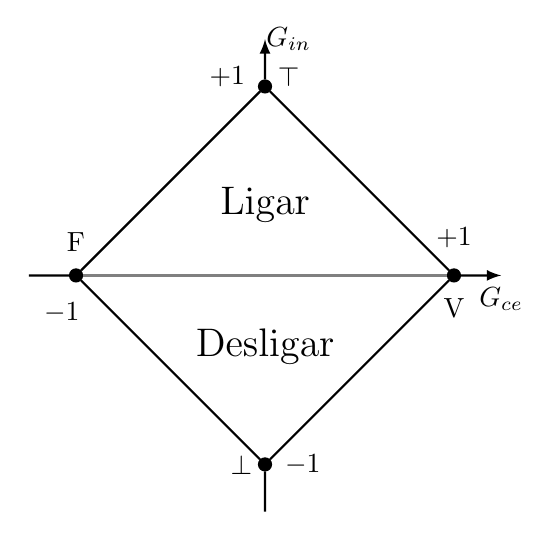
\begin{tikzpicture}[scale=0.60]
\tikzset{ >=latex, inner sep=0pt, outer sep=0pt,  }

%\draw [lightgray, dashed](0,0) grid (10,10);

\node [fill=black, circle] (V) at (9,5) {:};
\node [fill=black, circle] (F) at (1,5) {:};
\node [fill=black, circle] (T) at (5,9) {:};
\node [fill=black, circle] (L) at (5,1) {:};

\draw [->, thick] (V)   -- (10,5);
\draw [    thick] (0,5) -- (F);
\draw [->, thick] (T)   -- (5,10);
\draw [    thick] (5,0) -- (L);

\draw [thick] (V) -- (T);
\draw [thick] (T) -- (F);
\draw [thick] (F) -- (L);
\draw [thick] (L) -- (V);

\draw [gray,thick] (V) -- (F);

\node at (10,4.5) {$G_{ce}$};
\node at (5.5,10) {$G_{in}$};

\node at (4.2,9.2) {$+1$};
\node at (9.0,5.8) {$+1$};
\node at (5.8,1.0) {$-1$};
\node at (0.7,4.2) {$-1$};

\node at (9.0,4.3) {V};
\node at (1.0,5.7) {F};
\node at (5.5,9.2) {$\top$};
\node at (4.5,1.0) {$\bot$};

\node at (5.0,6.5) {\Large{Ligar}};
\node at (5.0,3.5) {\Large{Desligar}};

\end{tikzpicture}
\label{fig:reticuladoEtOnOff}

{\small Fonte: Próprio autor }
\end{figure}%%%%%%%%%%%%%%%%%%%%%%%%%%%%%%%%%%%%%%
%%%%%%%%%%%%%%%%%%%%%%%%%%%%%%%%%%%%%%%%%%%%%%%%%%





Utilizando o $G_{in}$ como variável condicionante:

\begin{itemize}
\item $Gin > 0 $: 
Para todas as combinaçãos de valores que produzam 
$\mu_0 > \mu_1$, 
ou seja, a variável de referência do sistema é 
maior do que a variável controlada,
o Grau de incerteza encontra-se na condição de 
\textit{Inconsistência}, conforme exposto na Equação 
\ref{eq:grauInconsistenciaIndefinicao}.

Substituindo $\mu$ por $\mu_0$ e 
$\lambda$ por $(1-\mu_1)$, 
utilizando a Equação \ref{eq:grauContradicao} 
( $Gin = \mu + \lambda - 1 $ )
temos:



\begin{equation}%%%%%%%%%%%%%%%%%%%%%%%%%%%%%%% Eq
Gin = \mu_0 + (1-\mu_1) -1
\end{equation}%%%%%%%%%%%%%%%%%%%%%%%%%%%%%%%%%%%%



simplificando temos então:



\begin{equation}%%%%%%%%%%%%%%%%%%%%%%%%%%%%%%% Eq
Gin = \mu_0 - \mu_1
\label{eq:gctmu0mu1}
\end{equation}%%%%%%%%%%%%%%%%%%%%%%%%%%%%%%%%%%%%



Supondo que o \emph{Valor desejado} indique que 
o valor da variável controlada é 25\% do valor máximo, 
o grau de evidência favorável 0 é $\mu_0 = 0,25$, 
enquanto que o \emph{sensor} indique que 
seu valor é de 20\% do valor máximo, 
o grau de evidência favorável 1 é $\mu_1 = 0,20$. 
Substituindo $\mu_0$ e $\mu_1$ em \ref{eq:gctmu0mu1}:



\begin{equation}%%%%%%%%%%%%%%%%%%%%%%%%%%%%%%% Eq
Gin = 0,25 - 0,20 = 0,05
\end{equation}%%%%%%%%%%%%%%%%%%%%%%%%%%%%%%%%%%%%



O ponto de operação do sistema 
localiza-se, então, acima da reta perfeitamente definida,
para todo grau de incerteza positivo, 
como é mostrado na Figura \ref{fig:gctpos}.



\item $Gin < 0 $: 
Para todas as combinações de valores que produzam 
$\mu_0 < \mu_1$, 
ou seja, a variável de referência do sistema é 
menor do que a variável controlada. 
O Grau de incerteza encontra-se na condição de 
\textit{Paracompleteza}, conforme exposto na Equação 
\ref{eq:grauInconsistenciaIndefinicao}.

Supondo agora que 
\emph{Valor desejado} continue indicando que 
o valor da variável controlada é 25\% do valor máximo,
o grau de evidência favorável 0 é $\mu_0 = 0,25$, 
mas o \emph{sensor} indique agora que
seu valor é de 30\% do valor máximo,
o grau de evidência favorável 1 é $\mu_1 = 0,30$.
Substituindo $\mu_0$ e $\mu_1$ em \ref{eq:gctmu0mu1}:



\begin{equation}%%%%%%%%%%%%%%%%%%%%%%%%%%%%%%% Eq
Gin = 0,25 - 0,30 = -0,05
\end{equation}%%%%%%%%%%%%%%%%%%%%%%%%%%%%%%%%%%%%



O ponto de operação do sistema 
localiza-se, então, abaixo da reta perfeitamente definida,
para todo grau de incerteza negativo,
como é mostrado na Figura \ref{fig:gctneg}.



\item $Gin = 0 $: 
Para todas as combinações de valores que produzam 
$\mu_0 = \mu_1$, 
ou seja, a variável de referência do sistema é 
igual a variável controlada,
não havendo necessidade de correções. 
O Grau de incerteza encontra-se na condição nula.

\end{itemize}




%%%%%%%%%%%%%%%%%%%%%%%%%%%%%%%%%%%%%%%%%%%%%%% Fg
\begin{figure}[!htb]%%%%%%%%%%%%%%%%%%%%%%%%%%%%%%
\centering
\caption{Representação do reticulado da LPA$E\tau$ para ação de controle Liga-Desliga}
\subfloat[$Gin$ positivo ($\mu_0 > \mu_1$)]{\label{fig:gctpos}

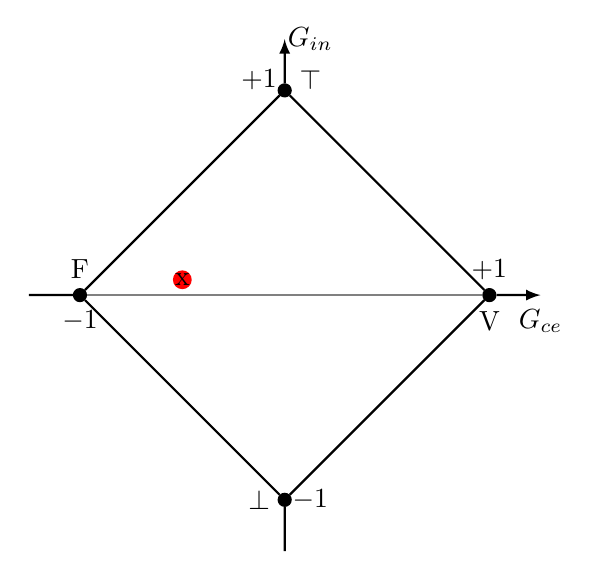
\begin{tikzpicture}[scale=0.65]
\tikzset{ >=latex, inner sep=0pt, outer sep=0pt,  }
%\draw [lightgray, dashed](0,0) grid (10,10);

\node [fill=black, circle] (V) at (9,5) {:};
\node [fill=black, circle] (F) at (1,5) {:};
\node [fill=black, circle] (T) at (5,9) {:};
\node [fill=black, circle] (L) at (5,1) {:};

\draw [->, thick] (V)   -- (10,5);
\draw [    thick] (0,5) -- (F);
\draw [->, thick] (T)   -- (5,10);
\draw [    thick] (5,0) -- (L);

\draw [thick] (V) -- (T);
\draw [thick] (T) -- (F);
\draw [thick] (F) -- (L);
\draw [thick] (L) -- (V);

\draw [gray,thick] (V) -- (F);

\node at (10,4.5) {$G_{ce}$};
\node at (5.5,10) {$G_{in}$};

\node at (4.5,9.2) {$+1$};
\node at (9.0,5.5) {$+1$};
\node at (5.5,1.0) {$-1$};
\node at (1.0,4.5) {$-1$};

\node at (9.0,4.5) {V};
\node at (1.0,5.5) {F};
\node at (5.5,9.2) {$\top$};
\node at (4.5,1.0) {$\bot$};

\node [fill=red, circle] (MU) at (3.0,5.3) {x};

\end{tikzpicture} }
\subfloat[$Gin$ negativo ($\mu_0<\mu_1$)]{\label{fig:gctneg}
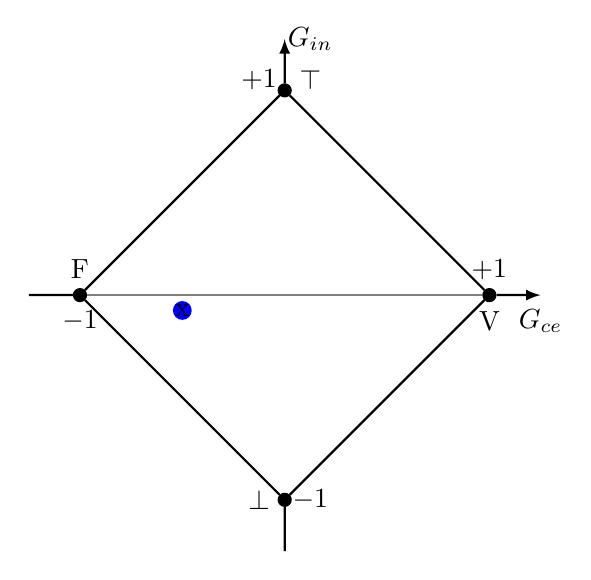
\begin{tikzpicture}[scale=0.65]
\tikzset{ >=latex, inner sep=0pt, outer sep=0pt,  }
%\draw [lightgray, dashed](0,0) grid (10,10);

\node [fill=black, circle] (V) at (9,5) {:};
\node [fill=black, circle] (F) at (1,5) {:};
\node [fill=black, circle] (T) at (5,9) {:};
\node [fill=black, circle] (L) at (5,1) {:};

\draw [->, thick] (V)   -- (10,5);
\draw [    thick] (0,5) -- (F);
\draw [->, thick] (T)   -- (5,10);
\draw [    thick] (5,0) -- (L);

\draw [thick] (V) -- (T);
\draw [thick] (T) -- (F);
\draw [thick] (F) -- (L);
\draw [thick] (L) -- (V);

\draw [gray,thick] (V) -- (F);

\node at (10,4.5) {$G_{ce}$};
\node at (5.5,10) {$G_{in}$};

\node at (4.5,9.2) {$+1$};
\node at (9.0,5.5) {$+1$};
\node at (5.5,1.0) {$-1$};
\node at (1.0,4.5) {$-1$};

\node at (9.0,4.5) {V};
\node at (1.0,5.5) {F};
\node at (5.5,9.2) {$\top$};
\node at (4.5,1.0) {$\bot$};

\node [fill=blue, circle] (MU1) at (3.0,4.7) {x};

\end{tikzpicture}}


{\small Fonte: Próprio autor}
\end{figure}%%%%%%%%%%%%%%%%%%%%%%%%%%%%%%%%%%%%%%
%%%%%%%%%%%%%%%%%%%%%%%%%%%%%%%%%%%%%%%%%%%%%%%%%%





Podemos então notar que 
a diferença existente entre os graus de evidência favoráveis 
é equivalente ao erro, 
como é denominado no sistema clássico de controle, 
mas que na representação da LPA$E\tau$ utilizando o reticulado,
pode ser considerado como 
o Grau de Incerteza, haja visto que,
na condição em que a variável controlada é igual a 
variável de referência, não há erro, e a inconsistência é zero, 
entretando se forem diferentes, 
tanto o erro quanto o grau de incerteza
serão não nulos. 

A opção pela ação de controle Liga-Desliga
é interessante do ponto de vista da velocidade 
de resposta ao degrau, 
porém apresenta uma oscilação que, 
a depender da dinâmica do sistema que está sendo trabalhado,
pode gerar uma amplitude maior do que o aceitável.
%como pôde ser visto na 
%Figura \ref{fig:acaoControleLigaDesliga}.

%Outra estratégia simples é a 
%utilização do sistema sem realimentação, 
%aplicando à saída o valor proporcional desejado.


%\section{A variável manipulada e a equivalência do controle em malha aberta}
\section{O Grau de Certeza ($G_{ce}$) como variável manipulada }

Assumindo não haver contradição, inconsistência, 
e para a Proposição adotada: 
\emph{"P: O acionamento do motor está ajustado para velocidade máxima."}, 
temos a Reta Perfeitamente Definida como referencial,
a Figura \ref{fig:gc25} então mostra o ponto de operação 
para uma velocidade de 25\% da proposição, 
e a Figura \ref{fig:gc90} mostra o ponto de operação
para a velocidade de 90\% da proposição.


%%%%%%%%%%%%%%%%%%%%%%%%%%%%%%%%%%%%%%%
%%%%%%%%%%%%%%%%%%%%%%%%%%%%%%%%%%%%%%%
\begin{figure}[!htb]
\centering
\caption{Representação do reticulado da LPA$E\tau$}
\subfloat[$Gce = -0,50 \ \ \ \mu_{ER} = 0,25$]{\label{fig:gc25}

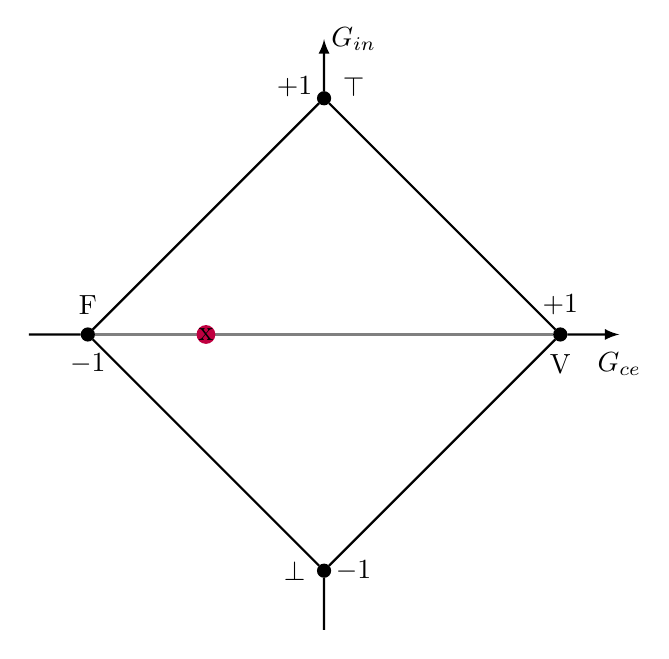
\begin{tikzpicture}[scale=0.75]
\tikzset{ >=latex, inner sep=0pt, outer sep=0pt,  }
%\draw [lightgray, dashed](0,0) grid (10,10);

\node [fill=black, circle] (V) at (9,5) {:};
\node [fill=black, circle] (F) at (1,5) {:};
\node [fill=black, circle] (T) at (5,9) {:};
\node [fill=black, circle] (L) at (5,1) {:};

\draw [->, thick] (V)   -- (10,5);
\draw [    thick] (0,5) -- (F);
\draw [->, thick] (T)   -- (5,10);
\draw [    thick] (5,0) -- (L);

\draw [thick] (V) -- (T);
\draw [thick] (T) -- (F);
\draw [thick] (F) -- (L);
\draw [thick] (L) -- (V);

\draw [gray,thick] (V) -- (F);

\node at (10,4.5) {$G_{ce}$};
\node at (5.5,10) {$G_{in}$};

\node at (4.5,9.2) {$+1$};
\node at (9.0,5.5) {$+1$};
\node at (5.5,1.0) {$-1$};
\node at (1.0,4.5) {$-1$};

\node at (9.0,4.5) {V};
\node at (1.0,5.5) {F};
\node at (5.5,9.2) {$\top$};
\node at (4.5,1.0) {$\bot$};

\node [fill=purple, circle] (MU) at (3.0,5.0) {x};

\end{tikzpicture} }
\subfloat[$Gce = 0,80 \ \ \ \mu_{ER} = 0,90$]{\label{fig:gc90}
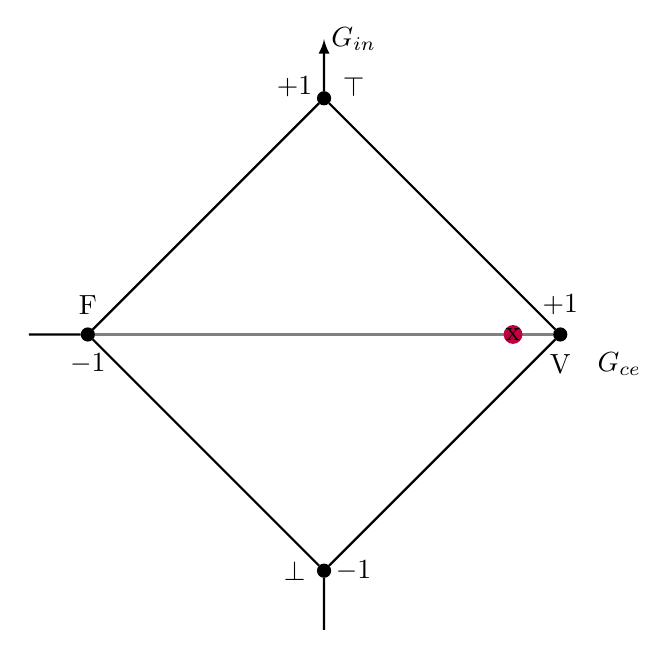
\begin{tikzpicture}[scale=0.75]
\tikzset{ >=latex, inner sep=0pt, outer sep=0pt,  }

\node [fill=black, circle] (V) at (9,5) {:};
\node [fill=black, circle] (F) at (1,5) {:};
\node [fill=black, circle] (T) at (5,9) {:};
\node [fill=black, circle] (L) at (5,1) {:};

\draw [    thick] (0,5) -- (F);
\draw [->, thick] (T)   -- (5,10);
\draw [    thick] (5,0) -- (L);

\draw [thick] (V) -- (T);
\draw [thick] (T) -- (F);
\draw [thick] (F) -- (L);
\draw [thick] (L) -- (V);

\draw [gray,thick] (V) -- (F);

\node at (10,4.5) {$G_{ce}$};
\node at (5.5,10) {$G_{in}$};

\node at (4.5,9.2) {$+1$};
\node at (9.0,5.5) {$+1$};
\node at (5.5,1.0) {$-1$};
\node at (1.0,4.5) {$-1$};

\node at (9.0,4.5) {V};
\node at (1.0,5.5) {F};
\node at (5.5,9.2) {$\top$};
\node at (4.5,1.0) {$\bot$};

\node [fill=purple, circle] (MU1) at (8.2,5.0) {x};

\end{tikzpicture}}

\label{fig:sistPrimeiraOrdem}

{\small Fonte: Próprio autor}
\end{figure}





%%%%%%%%%%%%%%%%%%%%%%%%%%%%%%%%%%%%%%%%%%%%%%%%%%
%%%%%%%%%%%%%%%%%%%%%%%%%%%%%%%%%%%%%%%%%%%%%%%%%%



\vspace{3cm}

Considerando o Grau de Incerteza nulo:

\begin{equation}
Gin = \mu + \lambda - 1 = 0 \rightarrow \mu = 1 - \lambda
\end{equation}

como $\mu_1 = 1 - \lambda$ e $\mu = \mu_0$:

\begin{equation}
\mu_0 = \mu_1
\label{eq:mu0eqmu1}
\end{equation}

e tal condição denota o ponto de operação
sobre a reta perfeitamente definida.
Assim a variação no processo de operação,
representado pelas anotações,
varia do estado
\emph{falso} para o
\emph{verdadeiro} no reticulado,
representando respectivamente
as condições de mínima e máxima velocidade,
sendo este intervalo o já denominado
Grau de Certeza (\emph{Gce}).

Como \emph{$G_{ce}$} excursiona no intervalo $[-1,1]$,
é realizada uma normalização e seu valor é
definido como Grau de Evidência Real $\mu_{ER}$,
assim, utilizando a Eq. \ref{eq:muer} e
substituindo $G_{ce}$ por $\mu - \lambda$, sendo $\mu = \mu_0$ e $\lambda = 1 - \mu_1$, temos que:


\begin{equation}
\mu_{ER} = \frac{G_{ce} + 1}{2} \rightarrow \mu_{ER} = \frac{(\mu_0 + \mu_1 - 1) + 1}{2} \rightarrow \mu_{ER} = \frac{\mu_0 + \mu_1}{2}
\label{eq:uermu0mu1}
\end{equation}

aplicando \ref{eq:mu0eqmu1} em \ref{eq:uermu0mu1}:

\begin{equation}
\mu_{ER} = \frac{\mu_0 + \mu_0}{2} = \frac{2.\mu_0}{2} = \mu_0
\end{equation}


Assim, adota-se como valor para a variável manipulada 
o valor $\mu_{ER}$, que é o próprio valor do 
grau de evidência favorável ($\mu_0$), 
e pode ser exemplificado na 
Figura \ref{fig:gc25} e na 
Figura \ref{fig:gc90}, 
respectivamente para valores de referência de 25\% e 90\%
do valor máximo da variável controlada.


\subsection{A equivalência ao controle em malha aberta}

Uma outra estratégia de controle simples, 
é a implementação equivalente a um controle em malha aberta,
onde é aplicado à entrada da planta, 
através da variável manipulada,
um valor proporcional ao valor desejado na saída,
que é a variável controlada, 
porém a planta controlada necessita apresentar um 
comportamento linear. 

Considerando o sistema linear,
pode-se então utilizar o $\mu_0$ como variável desejada, referência,
e o $\mu_{ER}$ como variável manipulada,
de forma equivalente a um sistema em malha aberta.

O controle em malha aberta apresenta simplicidade e facilidade mas
não atende a maioria dos usuários em suas necessidades,
sendo a presença de não linearidades,
um dos grandes problemas, 
comuns na maioria dos sistemas,
o que dificulta consideravelmente qualquer aplicação de controle.
Não havendo um rigor tão grande na aplicação,
uma certa parte dos sistemas pode ser controlado através de
uma configuração de malha aberta ou equivalente.


%%%%%%%%%%%%%%%%%%%%%%%%%%%%%%%%%%%%%%%%%%%%%%%%%%%%%%%%%%%%
%%%%%%%%%%%%%%%%%%%%%%%%%%%%%%%%%%%%%%%%%%%%%%%%%%%%%%%%%%%%

\section{Tratamento de não linearidades}

O tratamento de não linearidades não é contemplado pelos controles com lógica clássica,
sendo estes ajustados para operar em uma região linearizada do sistema,
e mudanças de região acompanham mudanças de configuração do controlador.
Utilizando a $LPAE\tau$ é possível prever e implementar o tratamento
das principais não linearidades diretamente no controlador,
sem que haja um rearranjo ou reconfiguração deste.

\subsection{A região de falsidade ( zona morta )}

O sistema possui uma região de operação 
que não é possível realizar o controle, 
pois é a região onde a inércia do sistema parado
impede a movimentação do eixo do motor para um baixo valor na variável manipulada,
em automação é costumeiramente denominada de Zona Morta, 
%o que deixa de acontecer em torno dos 10\% do valor do PWM.
e no reticulado em construção pode ser representada por uma região
próxima à falsidade.
O limiar da região de falsidade depende do sistema controlado,
e inicialmente, é estipulado um valor em torno dos 10\% do valor máximo de rotação,
como mostrado na Figura \ref{fig:zonaMorta}.





%%%%%%%%%%%%%%%%%%%%%%%%%%%%%%%%%%%%%%%%%%%%%%%%%%%%%%%%% Fg
\begin{figure}[!h]%%%%%%%%%%%%%%%%%%%%%%%%%%%%%%%%%%%%%%%%%%
\centering
\caption{Representação da zona morta no reticulado da LPA$E\tau$}
\begin{tikzpicture}[scale=0.80]
\tikzset{ >=latex, inner sep=0pt, outer sep=0pt,  }

%\draw [lightgray, dashed](0,0) grid (10,10);

\node [fill=black, circle] (V) at (9,5) {:};
\node [fill=black, circle] (F) at (1,5) {:};
\node [fill=black, circle] (T) at (5,9) {:};
\node [fill=black, circle] (L) at (5,1) {:};

\draw [->, thick] (V)   -- (10,5);
\draw [    thick] (0,5) -- (F);
\draw [->, thick] (T)   -- (5,10);
\draw [    thick] (5,0) -- (L);

\draw [thick] (V) -- (T);
\draw [thick] (T) -- (F);
\draw [thick] (F) -- (L);
\draw [thick] (L) -- (V);

\node at (10,4.5) {$G_{ce}$};
\node at (5.5,10) {$G_{in}$};

\node at (4.5,9.2) {$+1$};
\node at (9.0,5.5) {$+1$};
\node at (5.5,1.0) {$-1$};
\node at (1.0,4.5) {$-1$};

\node at (9.0,4.5) {V};
\node at (1.0,5.5) {F};
\node at (5.5,9.2) {$\top$};
\node at (4.5,1.0) {$\bot$};

\draw [fill, red,nearly transparent] (1.0,5.0) -- (1.5,5.5) -- (1.5,4.5) -- (1.0,5.0);
\draw [thick] (5.0,9.0) -- (1.0,5.0);
\draw [gray,thick] (V) -- (F);
\draw [dashed, red] (1.5,5.5) -- (1.5,4.5);
\end{tikzpicture}
\label{fig:zonaMorta}

{\small Fonte: Próprio autor }
\end{figure}
%%%%%%%%%%%%%%%%%%%%%%%%%%%%%%%%%%%%%%%%%%%%%%%%%%%%%%%%%%%%

A região de falsidade atende a uma condição de não linearidade que é bem comum de forma
consistente, sem a necessidade de tratamento externo ao controlador,
como é comum em controle clássico.



\subsection{A região de veracidade ( Saturação )}

A saturação de um acionamento ocorre quando a variável controlada atingiu o seu valor máximo
e a variável manipulada ainda não, sendo que qualquer incremento desta, até seu máximo valor,
não produz mais qualquer alteração na variável controlada.

A Figura \ref{fig:zonaSaturacao} evidencia a região de veracidade,
em que pode ocorrer a saturação do sistema. 


%%%%%%%%%%%%%%%%%%%%%%%%%%%%%%%%%%%%%%%%%%%%%%%%%%%%%%%%% Fg
\begin{figure}[!h]%%%%%%%%%%%%%%%%%%%%%%%%%%%%%%%%%%%%%%%%%%
\centering
\caption{Representação da saturação no reticulado da LPA$E\tau$}
\begin{tikzpicture}[scale=0.80]
\tikzset{ >=latex, inner sep=0pt, outer sep=0pt,  }

%\draw [lightgray, dashed](0,0) grid (10,10);

\node [fill=black, circle] (V) at (9,5) {:};
\node [fill=black, circle] (F) at (1,5) {:};
\node [fill=black, circle] (T) at (5,9) {:};
\node [fill=black, circle] (L) at (5,1) {:};

\draw [->, thick] (V)   -- (10,5);
\draw [    thick] (0,5) -- (F);
\draw [->, thick] (T)   -- (5,10);
\draw [    thick] (5,0) -- (L);

\draw [thick] (V) -- (T);
\draw [thick] (T) -- (F);
\draw [thick] (F) -- (L);
\draw [thick] (L) -- (V);

\node at (10,4.5) {$G_{ce}$};
\node at (5.5,10) {$G_{in}$};

\node at (4.5,9.2) {$+1$};
\node at (9.0,5.5) {$+1$};
\node at (5.5,1.0) {$-1$};
\node at (1.0,4.5) {$-1$};

\node at (9.0,4.5) {V};
\node at (1.0,5.5) {F};
\node at (5.5,9.2) {$\top$};
\node at (4.5,1.0) {$\bot$};

\draw [fill, purple,nearly transparent] (9.0,5.0) -- (8.5,5.5) -- (8.5,4.5) -- (9.0,5.0);
\draw [thick] (5.0,9.0) -- (1.0,5.0);
\draw [gray,thick] (V) -- (F);
\draw [dashed, red] (8.5,5.5) -- (8.5,4.5);
\end{tikzpicture}
\label{fig:zonaSaturacao}

{\small Fonte: Próprio autor }
\end{figure}
%%%%%%%%%%%%%%%%%%%%%%%%%%%%%%%%%%%%%%%%%%%%%%%%%%%%%%%%%%%%

Em função da normalização, conforme Equação \ref{eq:nomaliza},
a região de veracidade tende a zero,
no sentido que o sistema não apresenta saturação,
o máximo da variável manipulada produz o máximo da variável controlada.
Esta condição é produzida no processo de configuração das variáveis do sistema,
em que deve ser ajustado de acordo com as necessidades de implementação
específicos da aplicação.

\newpage



\subsection{A região de máxima inconsistência positiva/negativa tendendo a falsidade}
%(Travamento do motor ou falha do sensor)}

As regiões de máxima inconsistência positiva e negativa tendendo a falsidade
representam regiões de falha,
tanto por travamento do eixo do motor e acionamento involuntário,
quanto por falha do sensor de velocidade de rotação.

%A Figura \ref{fig:regiaoMaxInconsistencia} mostra
%as duas regiões para tratamento de falhas.





%%%%%%%%%%%%%%%%%%%%%%%%%%%%%%%%%%%%%%%
%%%%%%%%%%%%%%%%%%%%%%%%%%%%%%%%%%%%%%%
\begin{figure}[!htb]
\centering
\caption{Regiões de máxima inconsistência tendendo a falsidade}
\subfloat[Positiva: $\mu_0 > 0 e \mu_1 = 0$]{\label{fig:maxIncPos}

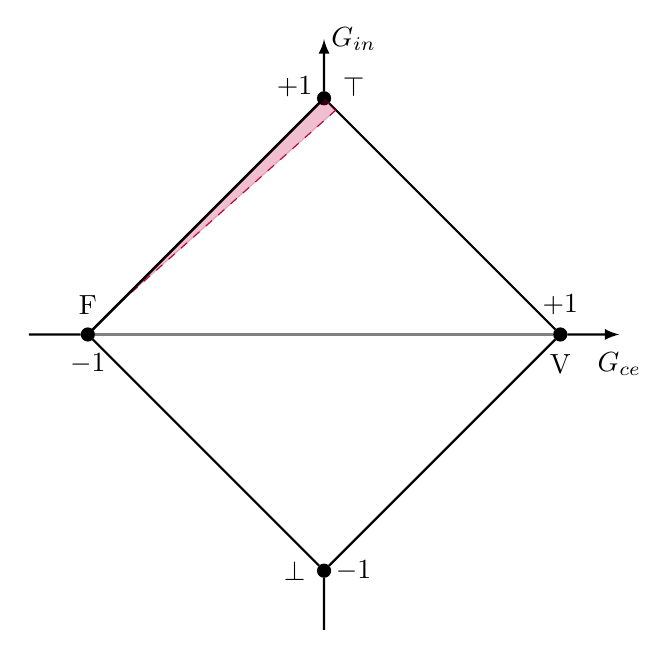
\begin{tikzpicture}[scale=0.75]
\tikzset{ >=latex, inner sep=0pt, outer sep=0pt,  }

%\draw [lightgray, dashed](0,0) grid (10,10);

\node [fill=black, circle] (V) at (9,5) {:};
\node [fill=black, circle] (F) at (1,5) {:};
\node [fill=black, circle] (T) at (5,9) {:};
\node [fill=black, circle] (L) at (5,1) {:};

\draw [->, thick] (V)   -- (10,5);
\draw [    thick] (0,5) -- (F);
\draw [->, thick] (T)   -- (5,10);
\draw [    thick] (5,0) -- (L);

\draw [thick] (V) -- (T);
\draw [thick] (T) -- (F);
\draw [thick] (F) -- (L);
\draw [thick] (L) -- (V);

\node at (10,4.5) {$G_{ce}$};
\node at (5.5,10) {$G_{in}$};

\node at (4.5,9.2) {$+1$};
\node at (9.0,5.5) {$+1$};
\node at (5.5,1.0) {$-1$};
\node at (1.0,4.5) {$-1$};

\node at (9.0,4.5) {V};
\node at (1.0,5.5) {F};
\node at (5.5,9.2) {$\top$};
\node at (4.5,1.0) {$\bot$};

\draw [fill, purple, nearly transparent] (1.5,5.5) -- (5.0,9.0) -- (5.2,8.8) -- (1.5,5.5);
\draw [dashed, purple] (5.2,8.8) -- (1.5,5.5);
\draw [thick] (5.0,9.0) -- (1.0,5.0);
\draw [gray,thick] (V) -- (F);

\end{tikzpicture} }
\subfloat[Negativa: $\mu_0 = 0 e \mu_1 > 0$]{\label{fig:maxIncNeg}
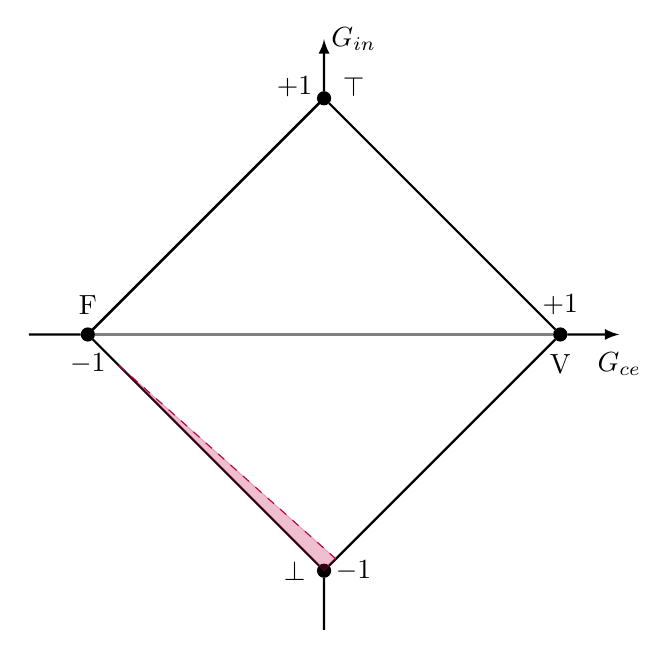
\begin{tikzpicture}[scale=0.75]
\tikzset{ >=latex, inner sep=0pt, outer sep=0pt,  }

%\draw [lightgray, dashed](0,0) grid (10,10);

\node [fill=black, circle] (V) at (9,5) {:};
\node [fill=black, circle] (F) at (1,5) {:};
\node [fill=black, circle] (T) at (5,9) {:};
\node [fill=black, circle] (L) at (5,1) {:};

\draw [->, thick] (V)   -- (10,5);
\draw [    thick] (0,5) -- (F);
\draw [->, thick] (T)   -- (5,10);
\draw [    thick] (5,0) -- (L);

\draw [thick] (V) -- (T);
\draw [thick] (T) -- (F);
\draw [thick] (F) -- (L);
\draw [thick] (L) -- (V);

\node at (10,4.5) {$G_{ce}$};
\node at (5.5,10) {$G_{in}$};

\node at (4.5,9.2) {$+1$};
\node at (9.0,5.5) {$+1$};
\node at (5.5,1.0) {$-1$};
\node at (1.0,4.5) {$-1$};

\node at (9.0,4.5) {V};
\node at (1.0,5.5) {F};
\node at (5.5,9.2) {$\top$};
\node at (4.5,1.0) {$\bot$};

\draw [fill, purple, nearly transparent] (1.5,4.5) -- (5.0,1.0) -- (5.2,1.2) -- (1.5,4.5);
\draw [dashed, purple] (5.2,1.2) -- (1.5,4.5);
\draw [thick] (5.0,9.0) -- (1.0,5.0);
\draw [gray,thick] (V) -- (F);

\end{tikzpicture}}

\label{fig:regiaoMaxInconsistencia}

{\small Fonte: Próprio autor}
\end{figure}



%A Figura \ref{fig:maxIncPos} mostra a região de operação para a condição
%em que o $\mu_0$ apresenta valor diferente de nulo e o
%$\mu_1$ igual a zero ou menor do que um valor limiar,
%que pode ser definido a depender da aplicação.

%De forma análoga, a Figura \ref{fig:maxIncNeg} mostra a região de oparação para a condição
%em que o $\mu_0$ apresenta valor nulo ou próximo a zero,
%menor do que o limiar estabelecido para a aplicação e o
%$\mu_1$ apresente valor nulo.



%%%%%%%%%%%%%%%%%%%%%%%%%%%%%%%%%%%%%%%%%%%%%%%%%%
%%%%%%%%%%%%%%%%%%%%%%%%%%%%%%%%%%%%%%%%%%%%%%%%%%

%\subsubsection{Tratamento de falha}


O sistema pode falhar apresentando um travamento inesperado do eixo do motor,
produzindo, para o grau de evidência contrário,
que está associado ao sensor, um valor máximo,
pelo seu caráter complementar, equivalendo a velocidade nula do eixo do motor,
para o grau de evidência favorável não nulo, ou seja,
para uma velocidade desejada diferente de zero.

Outra possibilidade de falha é caso o sensor de velocidade apresente falha,
indicando sempre uma velocidade nula,
tanto pela falta de um acoplamento sensor/disco de leitura quanto pela
falta de sinal elétrico ou alimentação.

A Figura \ref{fig:maxIncPos} mostra a região do reticulado que pode
evidencia as anormalidades citadas,
podendo produzir uma tomada de decisão no acionamento e na sinalização do sistema.


Nesta condição o controlador pode tomar a decisão de 
desligar o sistema controlado, 
levá-lo a condição de falha e 
sinalizar ao operador a irregularidade, 
a depender do tipo de sistema a ser controlado.



%\subsection{A região de máxima inconsistência negativa tendendo a falsidade (acionamento involuntário)}

Na eventualidade de haver uma falha do circuito de acionamento,
produzindo um sinal de acionamento indevido do motor,
este produz no sensor um sinal diferente de zero,
tornando o grau de evidência contrário tendendo a zero e
o grau de evidência favorável nulo,
pois não houve acioamento voluntário.
A região para tratamento de acionamento involuntário
é apresentada na Figura \ref{fig:maxIncNeg}.

Esta é uma falha crítica do hardware que não pode ser tratada pelo controlador,
pois a variável manipulada está comprometida por
um sinal eventual de falha de hardware,
mas pode ser sinalizada e de alguma forma tratado pelo operador do sistema.


%%%%%%%%%%%%%%%%%%%%%%%%%%%%%%%%%%%%%%%%%%%%%%% Fg
%\begin{figure}[!h]%%%%%%%%%%%%%%%%%%%%%%%%%%%%%%%%
%\centering
%\caption{Representação da região de máxima inconsistência positiva tendendo a falsidade }
%\begin{tikzpicture}[scale=0.80]
%\tikzset{ >=latex, inner sep=0pt, outer sep=0pt,  }

%\draw [lightgray, dashed](0,0) grid (10,10);

%\node [fill=black, circle] (V) at (9,5) {:};
%\node [fill=black, circle] (F) at (1,5) {:};
%\node [fill=black, circle] (T) at (5,9) {:};
%\node [fill=black, circle] (L) at (5,1) {:};

%\draw [->, thick] (V)   -- (10,5);
%\draw [    thick] (0,5) -- (F);
%\draw [->, thick] (T)   -- (5,10);
%\draw [    thick] (5,0) -- (L);

%\draw [thick] (V) -- (T);
%\draw [thick] (T) -- (F);
%\draw [thick] (F) -- (L);
%\draw [thick] (L) -- (V);

%\node at (10,4.5) {$G_{ce}$};
%\node at (5.5,10) {$G_{in}$};

%\node at (4.5,9.2) {$+1$};
%\node at (9.0,5.5) {$+1$};
%\node at (5.5,1.0) {$-1$};
%\node at (1.0,4.5) {$-1$};

%\node at (9.0,4.5) {V};
%\node at (1.0,5.5) {F};
%\node at (5.5,9.2) {$\top$};
%\node at (4.5,1.0) {$\bot$};

%\draw [fill, purple, nearly transparent] (1.5,5.5) -- (5.0,9.0) -- (5.2,8.8) -- (1.5,5.5);
%\draw [dashed, purple] (5.2,8.8) -- (1.5,5.5);
%\draw [thick] (5.0,9.0) -- (1.0,5.0);
%\draw [gray,thick] (V) -- (F);
%\end{tikzpicture}
%\label{fig:travamentoEixo}

%{\small Fonte: Próprio autor }
%\end{figure}
%%%%%%%%%%%%%%%%%%%%%%%%%%%%%%%%%%%%%%%%%%%%%%%%%%






%%%%%%%%%%%%%%%%%%%%%%%%%%%%%%%%%%%%%%%%%%%%%%% Fg
%\begin{figure}[!h]%%%%%%%%%%%%%%%%%%%%%%%%%%%%%%%%
%\centering
%\caption{Representação da região de máxima inconsistência positiva tendendo a falsidade }
%\begin{tikzpicture}[scale=0.80]
%\tikzset{ >=latex, inner sep=0pt, outer sep=0pt,  }

%\draw [lightgray, dashed](0,0) grid (10,10);

%\node [fill=black, circle] (V) at (9,5) {:};
%\node [fill=black, circle] (F) at (1,5) {:};
%\node [fill=black, circle] (T) at (5,9) {:};
%\node [fill=black, circle] (L) at (5,1) {:};

%\draw [->, thick] (V)   -- (10,5);
%\draw [    thick] (0,5) -- (F);
%\draw [->, thick] (T)   -- (5,10);
%\draw [    thick] (5,0) -- (L);

%\draw [thick] (V) -- (T);
%\draw [thick] (T) -- (F);
%\draw [thick] (F) -- (L);
%\draw [thick] (L) -- (V);

%\node at (10,4.5) {$G_{ce}$};
%\node at (5.5,10) {$G_{in}$};

%\node at (4.5,9.2) {$+1$};
%\node at (9.0,5.5) {$+1$};
%\node at (5.5,1.0) {$-1$};
%\node at (1.0,4.5) {$-1$};

%\node at (9.0,4.5) {V};
%\node at (1.0,5.5) {F};
%\node at (5.5,9.2) {$\top$};
%\node at (4.5,1.0) {$\bot$};

%\draw [fill, purple, nearly transparent] (1.5,4.5) -- (5.0,1.0) -- (5.2,1.2) -- (1.5,4.5);
%\draw [dashed, purple] (5.2,1.2) -- (1.5,4.5);
%\draw [thick] (5.0,9.0) -- (1.0,5.0);
%\draw [gray,thick] (V) -- (F);
%\end{tikzpicture}
%\label{fig:acionaInvoluntarioEixo}

%{\small Fonte: Próprio autor }
%\end{figure}
%%%%%%%%%%%%%%%%%%%%%%%%%%%%%%%%%%%%%%%%%%%%%%%%%%





\section{A região de incerteza (trivialidade) admitida }

Em torno da reta perfeitamente definida,
eixo que denota o Grau de Certeza ($G_{ce}$),
ou para a região em que o Grau de Incerteza é próximo a zero
o suficiente para produzir um erro aceitável,
a essa região é denominada de Região de Incerteza (Trivialidade) Admitida.

Essa região é mostrada na Figura \ref{fig:zonaIncertezaAdmitida},
podendo os limiares superior e inferior apresentar distâncias diferentes
em relação ao zero do $G_{in}$. 


%%%%%%%%%%%%%%%%%%%%%%%%%%%%%%%%%%%%%%%%%%%%%%%%%%%%%%%%% Fg
\begin{figure}[!h]%%%%%%%%%%%%%%%%%%%%%%%%%%%%%%%%%%%%%%%%%%
\centering
\caption{Representação da região de Incerteza Admitida}
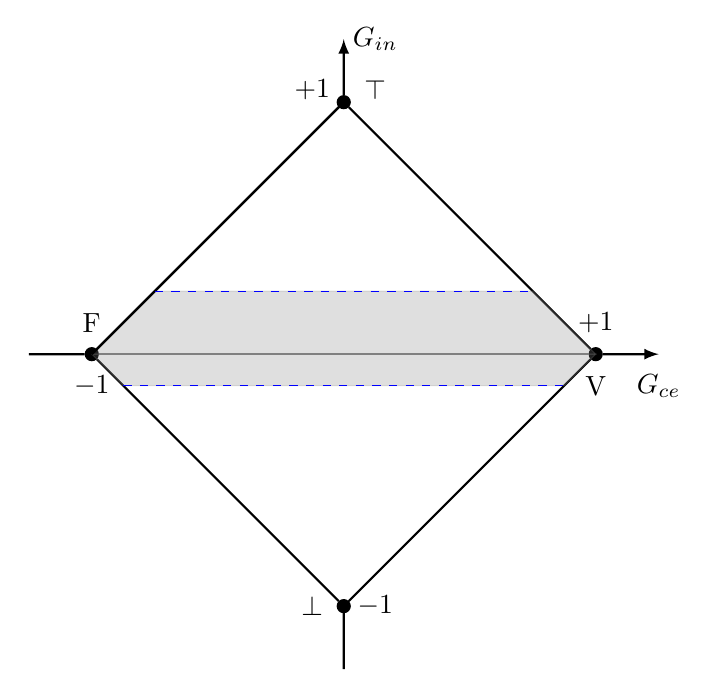
\begin{tikzpicture}[scale=0.80]
\tikzset{ >=latex, inner sep=0pt, outer sep=0pt,  }

%\draw [lightgray, dashed](0,0) grid (10,10);

\node [fill=black, circle] (V) at (9,5) {:};
\node [fill=black, circle] (F) at (1,5) {:};
\node [fill=black, circle] (T) at (5,9) {:};
\node [fill=black, circle] (L) at (5,1) {:};

\draw [->, thick] (V)   -- (10,5);
\draw [    thick] (0,5) -- (F);
\draw [->, thick] (T)   -- (5,10);
\draw [    thick] (5,0) -- (L);

\draw [thick] (V) -- (T);
\draw [thick] (T) -- (F);
\draw [thick] (F) -- (L);
\draw [thick] (L) -- (V);

\node at (10,4.5) {$G_{ce}$};
\node at (5.5,10) {$G_{in}$};

\node at (4.5,9.2) {$+1$};
\node at (9.0,5.5) {$+1$};
\node at (5.5,1.0) {$-1$};
\node at (1.0,4.5) {$-1$};

\node at (9.0,4.5) {V};
\node at (1.0,5.5) {F};
\node at (5.5,9.2) {$\top$};
\node at (4.5,1.0) {$\bot$};

\draw [fill, gray,nearly transparent] (1.0,5.0) -- (2.0,6.0) -- (8.0,6.0) -- (9.0,5.0) -- (1.0,5.0);
\draw [fill, gray,nearly transparent] (1.0,5.0) -- (1.5,4.5) -- (8.5,4.5) -- (9.0,5.0) -- (1.0,5.0);
\draw [thick] (5.0,9.0) -- (1.0,5.0);
\draw [gray,thick] (V) -- (F);
\draw [dashed, blue] (2.0,6.0) -- (8.0,6.0);
\draw [dashed, blue] (1.5,4.5) -- (8.5,4.5);
\end{tikzpicture}
\label{fig:zonaIncertezaAdmitida}

{\small Fonte: Próprio autor }
\end{figure}
%%%%%%%%%%%%%%%%%%%%%%%%%%%%%%%%%%%%%%%%%%%%%%%%%%%%%%%%%%%%









\subsection{A incerteza admitida como histerese ou erro de regime estacionário}

Como essa região é a admissão de uma incerteza,
ela pode conter uma não linearidade,
denominada em automação de histerese,
que de um modo geral é produzida pela diferença entre resposta
no avanço e retrocesso do sinal da variável manipulada,
ou seja,
os caminhos de excursão na subida do sinal e na descida diferem.

Ao entrar em estabilidade,
é possível que haja uma diferença em relação a referência,
e tal diferença é denominada de erro de regime estacionário.

A incerteza admitida deve possuir limiar que contemple
a histerese ou o erro de regime estacionário
a depender do sistema controlado. 


\subsection{ A região de operação }

A região de incerteza admitida é a região de operação para o sistema em regime, 
quando ele entra em estabilidade,
e é estipulado um valor de grau de incerteza admissível que 
pode ser alterado posteriormente a testes empíricos.

O grau de incerteza admitido está definido entre
o intervalo menor ou igual a 0,1 ($Gin \le 0,1$) 
e maior ou igual a -0,05 ($Gin \ge -0,05$).

%Assumindo um valor inicial para
%a variável manipulada equivalente a um controle em malha aberta, sendo
%assim a resposta do controlador é o próprio $\mu_0$.
%como mostra a Figura \ref{fig:regiaoAtiva}.



A variável manipulada assume o valor da entrada $\mu_0$,
enviando à saída um valor proporcional ao valor desejado.
Mas como a relação entre o valor de referência e a 
velocidade de rotação do motor não é perfeitamente linear,
para cada região ou patamar da velocidade do motor,
pode haver um erro considerável,
inclusive sendo maior do que o valor permitido pela 
tolerância. 

Assim para reduzir o grau de incerteza
em decorrência dessa não linearidade, 
é somado ao $\mu_0$ um valor de correção denominado $\delta$(delta).

Então a representação do reticulado da LPA$E\tau$ 
fica conforme é apresentada na Figura \ref{fig:regiaoAtivaMuDelta}. 





%%%%%%%%%%%%%%%%%%%%%%%%%%%%%%%%%%%%%%%%%%%%%% Fig
\begin{figure}[!h]%%%%%%%%%%%%%%%%%%%%%%%%%%%%%%%%
\centering
\caption{Representação da região ativa no reticulado acrescido do $\delta$}
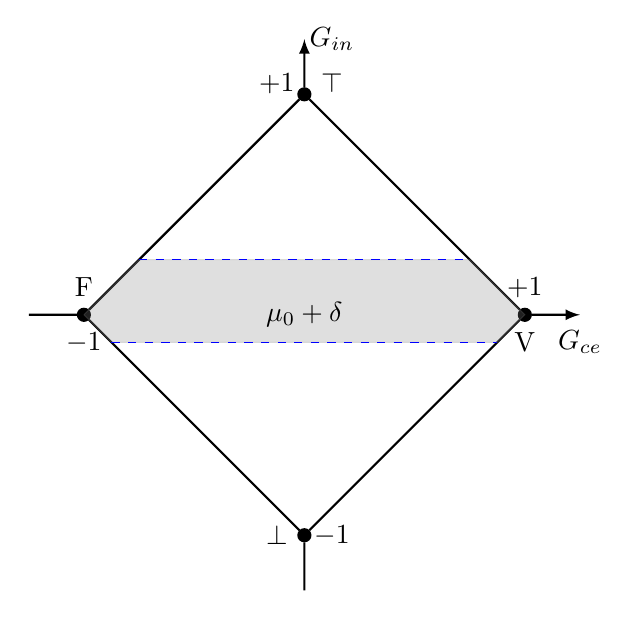
\begin{tikzpicture}[scale=0.70]
\tikzset{ >=latex, inner sep=0pt, outer sep=0pt,  }

%\draw [lightgray, dashed](0,0) grid (10,10);

\node [fill=black, circle] (V) at (9,5) {:};
\node [fill=black, circle] (F) at (1,5) {:};
\node [fill=black, circle] (T) at (5,9) {:};
\node [fill=black, circle] (L) at (5,1) {:};

\draw [->, thick] (V)   -- (10,5);
\draw [    thick] (0,5) -- (F);
\draw [->, thick] (T)   -- (5,10);
\draw [    thick] (5,0) -- (L);

\draw [thick] (V) -- (T);
\draw [thick] (T) -- (F);
\draw [thick] (F) -- (L);
\draw [thick] (L) -- (V);

\node at (10,4.5) {$G_{ce}$};
\node at (5.5,10) {$G_{in}$};

\node at (4.5,9.2) {$+1$};
\node at (9.0,5.5) {$+1$};
\node at (5.5,1.0) {$-1$};
\node at (1.0,4.5) {$-1$};

\node at (9.0,4.5) {V};
\node at (1.0,5.5) {F};
\node at (5.5,9.2) {$\top$};
\node at (4.5,1.0) {$\bot$};


%\draw [fill, gray,nearly transparent] (1.0,5.0) -- (2.0,6.0) -- (8.0,6.0) -- (9.0,5.0) -- (1.0,5.0);
%\draw [fill, gray,nearly transparent] (1.0,5.0) -- (1.5,4.5) -- (8.5,4.5) -- (9.0,5.0) -- (1.0,5.0);
\draw [fill, gray,nearly transparent] (1.0,5.0) -- (2.0,6.0) -- (8.0,6.0) -- (9.0,5.0) -- (8.5,4.5)--(1.5,4.5) -- (1.0,5.0);
%\draw [thick] (5.0,9.0) -- (1.0,5.0);
%\draw [gray,thick] (V) -- (F);
\draw [dashed, blue] (2.0,6.0) -- (8.0,6.0);
\draw [dashed, blue] (1.5,4.5) -- (8.5,4.5);

\node at (5.0,5.0) {$\mu_0 + \delta$};

\end{tikzpicture}
\label{fig:regiaoAtivaMuDelta}

{\small Fonte: Próprio autor }
\end{figure}
%%%%%%%%%%%%%%%%%%%%%%%%%%%%%%%%%%%%%%%%%%%%%%%%%%





A região ativa então pode ser dividida em 
tantas partes quantas forem necessárias 
para garantir um $\delta$ satisfatório para tal região,
pois esse valor não garante erro nulo para toda extensão
possível.



Para gerar um divisão de valores alvo, 
em que o erro seja de no máximo 5\%, 
foi gerada uma tabela que tem como valor inicial
o 10, pois é assumido que para o sistema em estudo,
valores abaixo são considerados zona morta.

A cada incremento de 10\% aproximadamente, 
é gerado o próximo elemento, até o máximo valor menor do que
100, equivalente à 100\% do valor máximo de saída.


%%%%%%%%%%%%%%%%%%%%%%%%%%%%%%%%%%%%%%%%%%%%%% Fig
\begin{figure}[!h]%%%%%%%%%%%%%%%%%%%%%%%%%%%%%%%%
\centering
\caption{Representação da região ativa no reticulado acrescido de subdivisões $\delta$}
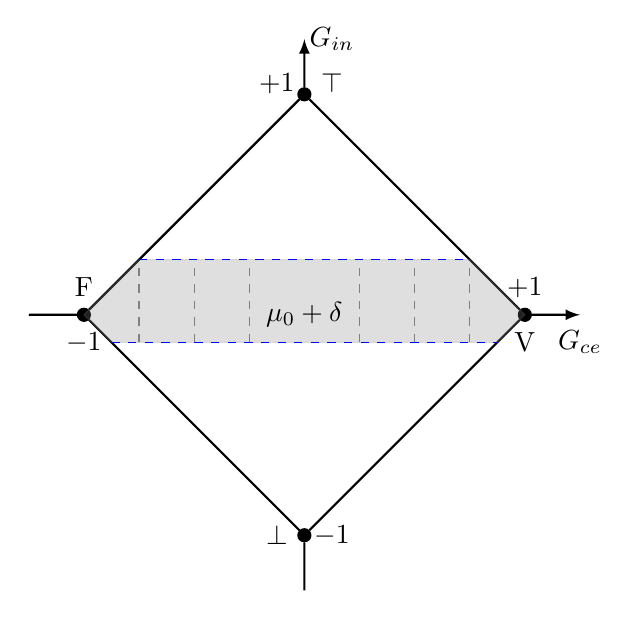
\begin{tikzpicture}[scale=0.70]
\tikzset{ >=latex, inner sep=0pt, outer sep=0pt,  }

%\draw [lightgray, dashed](0,0) grid (10,10);

\node [fill=black, circle] (V) at (9,5) {:};
\node [fill=black, circle] (F) at (1,5) {:};
\node [fill=black, circle] (T) at (5,9) {:};
\node [fill=black, circle] (L) at (5,1) {:};

\draw [->, thick] (V)   -- (10,5);
\draw [    thick] (0,5) -- (F);
\draw [->, thick] (T)   -- (5,10);
\draw [    thick] (5,0) -- (L);

\draw [thick] (V) -- (T);
\draw [thick] (T) -- (F);
\draw [thick] (F) -- (L);
\draw [thick] (L) -- (V);

\node at (10,4.5) {$G_{ce}$};
\node at (5.5,10) {$G_{in}$};

\node at (4.5,9.2) {$+1$};
\node at (9.0,5.5) {$+1$};
\node at (5.5,1.0) {$-1$};
\node at (1.0,4.5) {$-1$};

\node at (9.0,4.5) {V};
\node at (1.0,5.5) {F};
\node at (5.5,9.2) {$\top$};
\node at (4.5,1.0) {$\bot$};


\draw [fill, gray,nearly transparent] (1.0,5.0) -- (2.0,6.0) -- (8.0,6.0) -- (9.0,5.0) -- (8.5,4.5)--(1.5,4.5) -- (1.0,5.0);
\draw [gray, dashed] (2.0,4.5) -- (2.0,6.0);
\draw [gray, dashed] (3.0,4.5) -- (3.0,6.0);
\draw [gray, dashed] (4.0,4.5) -- (4.0,6.0);
\draw [gray, dashed] (6.0,4.5) -- (6.0,6.0);
\draw [gray, dashed] (7.0,4.5) -- (7.0,6.0);
\draw [gray, dashed] (8.0,4.5) -- (8.0,6.0);
%\draw [gray,thick] (V) -- (F);
\draw [dashed, blue] (2.0,6.0) -- (8.0,6.0);
\draw [dashed, blue] (1.5,4.5) -- (8.5,4.5);

\node at (5.0,5.0) {$\mu_0 + \delta$};

\end{tikzpicture}
\label{fig:regiaoAtivaMuDeltaN}

{\small Fonte: Próprio autor }
\end{figure}
%%%%%%%%%%%%%%%%%%%%%%%%%%%%%%%%%%%%%%%%%%%%%%%%%%



Sendo assim segue a 
Tabela \ref{tab:correcaoDelta} 
com os respectivos valores alvo, 
os limites inferiores e superiores, 
que são calculados baseados em decremento de 5\% e
incremento de 5\%, respectivamente, ao valor alvo.

Para todo valor alvo, uma variação positiva ou negativa
de 5\% está enquadrada dentro dos limites motrados na Tabela.

Esses intervalos abrangem todo o intervalo entre 
o valor 10 e o 100, mínimo e máximo, 
de modo a qualquer valor desejado fique 
dentro de algum intervalo, 
e possua um valor alvo bem próximo.


\begin{table}[h]
\centering
\caption{Valores de correção para a condição de inconsistência}
\label{tab:correcaoDelta}

\begin{tabular}{c|c|c||c}
\hline
%Intervalo de amostras  &  erro médio relativo \\ \hline
Limite Inferior & Alvo & Limite Superior & Valor de Correção\\ \hline
\hline
%0 a 1 $\tau$ & 83,40 \% \\ \hline
 9,5 & 10 & 10,5 & $\delta_0$ \\ \hline
10,5 & 11 & 11,5 & $\delta_1$ \\ \hline
11,5 & 12 & 12,5 & $\delta_2$ \\ \hline
12,5 & 13 & 14,0 & $\delta_3$ \\ \hline
14,0 & 15 & 15,5 & $\delta_4$ \\ \hline
15,5 & 16 & 17,0 & $\delta_5$ \\ \hline
17,0 & 18 & 19,0 & $\delta_6$ \\ \hline
19,0 & 20 & 21,0 & $\delta_7$ \\ \hline
21,0 & 22 & 23,0 & $\delta_8$ \\ \hline
23,4 & 24 & 25,4 & $\delta_9$ \\ \hline
25,4 & 27 & 28,4 & $\delta_{10}$ \\ \hline
28,4 & 30 & 31,4 & $\delta_{11}$ \\ \hline
31,4 & 33 & 34,4 & $\delta_{12}$ \\ \hline
34,4 & 36 & 37,4 & $\delta_{13}$ \\ \hline
37,4 & 39 & 40,9 & $\delta_{14}$ \\ \hline
40,9 & 43 & 44,9 & $\delta_{15}$ \\ \hline
44,9 & 47 & 48,9 & $\delta_{16}$ \\ \hline
48,9 & 51 & 53,4 & $\delta_{17}$ \\ \hline
53,4 & 56 & 58,9 & $\delta_{18}$ \\ \hline
58,9 & 62 & 64,9 & $\delta_{19}$ \\ \hline
64,9 & 68 & 71,3 & $\delta_{20}$ \\ \hline
71,3 & 75 & 78,3 & $\delta_{21}$ \\ \hline
78,3 & 82 & 86,3 & $\delta_{22}$ \\ \hline
86,3 & 91 &100,0 & $\delta_{23}$ \\ \hline

\end{tabular}

{\vspace{0.2cm} \small Fonte: Próprio autor}
\end{table}


Para cada valor alvo, há um valor $\delta$ associado, 
que é um valor de correção.
Tomando como exemplo o valor de referência 25\%, 
no momento inicial há uma grande inconsistência,
então o reticulado assume na saída o valor 1, 
do estado de valor máximo apresentado na 
Figura \ref{fig:regiaoAtivaMuDelta}.
Ao sistema então é aplicada a potência máxima, 
vencendo a inércia do repouso.
O grau de incerteza é reduzido conforme 
o sistema se aproxima do ponto de operação desejado,
e quando o seu valor é menor do que 
o parâmetro de limite, nesse caso estabelecido em 0,10,
a saída assume o valor equivalente ao $\mu_0$, ou seja,
o valor de referência, então: $\mu_0 = 0,25$, porém 
é acrescido o valor do $\delta_9$, 
que refere-se ao intervalo em que se encontra o 25\%.

Assim a saída do controlador LPA$E\tau$ é 
$\mu_0 + \delta_9$
para um valor de referência de 25\% do valor máximo.





%%%%%%%%%%%%%%%%%%%%%%%%%%%%%%%%%%%%%%%%%%%%%%%%%%%%%%%%%%%%
%%%%%%%%%%%%%%%%%%%%%%%%%%%%%%%%%%%%%%%%%%%%%%%%%%%%%%%%%%%%



\newpage
\subsubsection{O fator de correção $\delta$}

O fator de correção $\delta$ tem a finalidade de corrigir a variável
manipulada de modo a zerar a diferença entre a variável controlada e a
variável de referência. A correção aqui empregada é de ajuste fino da
variável manipulada.

A correção se dá por um algorítmo que implementa um filtro de média móvel
tendo como elemento de cálculo o Grau de Incerteza,
como mostra a Figura \ref{fig:diagramaBlocosLPAEtDelta}.



\begin{figure}[!h]%%%%%%%%%%%%%%%%%%%%%%%%%%%%%%%%fg
\centering
\caption{Diagrama de blocos do controle com cálculo do Delta}
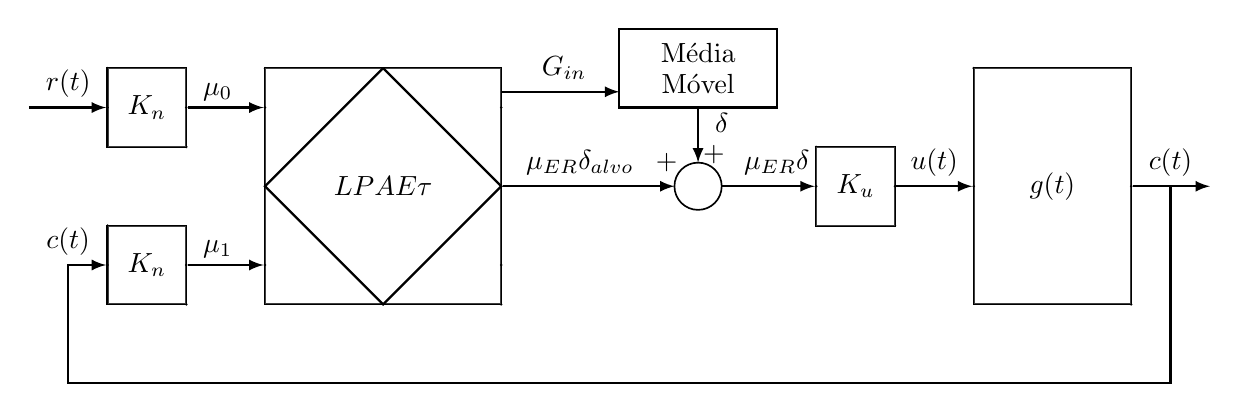
\begin{tikzpicture}[scale=1.0]
\tikzset{ >=latex, inner sep=0pt, outer sep=0pt,  }

%\draw [lightgray, dashed](0,0) grid (15,4.2);

%%% Blocos 

% Kn normalização rps -> 0..1
\node [fill=black, circle] (KSP0) at (1.0,4.0) { };
\node [fill=black, circle] (KSP1) at (2.0,3.0) { };
\draw[thick] (KSP0) rectangle (KSP1);
\fill[white, nearly transparent] (KSP0) rectangle (KSP1);
\node [fill=black, circle] (KSPin)  at (1.0,3.5) { }; 
\node [fill=black, circle] (KSPout) at (2.0,3.5) { }; 
\node (Kn1) at (1.5,3.5) {$K_n$};

% Kn Sensor
\node [fill=black, circle] (KS0) at (1.0,2.0) { };
\node [fill=black, circle] (KS1) at (2.0,1.0) { };
\draw[thick] (KS0) rectangle (KS1);
\fill[white, nearly transparent] (KS0) rectangle (KS1);
\node [fill=black, circle] (KSin)  at (1.0,1.5) { };
\node [fill=black, circle] (KSout) at (2.0,1.5) { };
\node (Kn2) at (1.5,1.5) {$K_n$};

% LPAEt
\node [fill=black, circle] (LPA0) at (3,4.0) { };
\node [fill=black, circle] (LPA1) at (6,1.0) { };
\draw[thick] (LPA0) rectangle (LPA1);
\fill[white, nearly transparent] (LPA0) rectangle (LPA1);
\draw [thick] (4.5,4.0) -- (6.0,2.5) -- (4.5,1.0) -- (3.0,2.5) -- (4.5,4.0);
\node (LPA2v) at (4.5,2.5) {$LPAE\tau$};
\node [fill=black, circle] (LPAu0)  at (3.0,3.5) { };
\node [fill=black, circle] (LPAu1)  at (3.0,1.5) { };
\node [fill=black, circle] (LPAgc)  at (6.0,3.5) { };
\node [fill=black, circle] (LPAs)   at (6.0,2.5) { };
\node [fill=black, circle] (LPAgct) at (6.0,1.5) { };
\node (LPA2vu0)  at (2.4,3.7) {$\mu _0$};
\node (LPA2vu1)  at (2.4,1.7) {$\mu _1$};

% Kn u(t)
\node [fill=black, circle] (KU0) at (10.0,3.0) { };
\node [fill=black, circle] (KU1) at (11.0,2.0) { };
\draw[thick] (KU0) rectangle (KU1);
\fill[white, nearly transparent] (KU0) rectangle (KU1);
\node [fill=black, circle] (KUin)  at (10.0,2.5) { };
\node [fill=black, circle] (KUout) at (11.0,2.5) { };
\node (Ku2) at (10.5,2.5) {$K_u$};


% Planta
\node [fill=black, circle] (GT0) at (12,4.0) { };
\node [fill=black, circle] (GT1) at (14,1.0) { };
\draw[thick] (GT0) rectangle (GT1);
\fill[white, nearly transparent] (GT0) rectangle (GT1);
\node [fill=black, circle] (GTin)  at (12.0,2.5) { };
\node [fill=black, circle] (GTout) at (14.0,2.5) { };
\node (planta) at (13.0,2.5) {$g(t)$};



%%% Linhas 

% set point
\draw [->, thick] (0.0,3.5) -- (KSPin);
\node (rt) at (0.5,3.8) {$r(t)$};

% GT -> fim
\draw [->, thick] (GTout) -- (15,2.5);
\node (ct) at (14.5,2.8) {$c(t)$};
\node (ct) at (0.5,1.8) {$c(t)$};

% normalização 0..1 -> LPA2v u0
\draw [->, thick] (KSPout) -- (LPAu0);

% normalização 0..1 -> LPA2v u1
\draw [->, thick] (KSout) -- (LPAu1);

% LPAEt -> Ku
\draw [->, thick] (LPAs) -- (8.2,2.5);
\draw [->, thick] (8.8,2.5) -- (KUin);
\node (ut) at (9.5,2.8) {$\mu_{ER}\delta$};
\node (ut) at (7.0,2.8) {$\mu_{ER}\delta_{alvo}$};

% Ku -> GT
\draw [->, thick] (KUout) -- (GTin);
\node (ut) at (11.5,2.8) {$u(t)$};

% GT -> Kn Sensor
\draw [->, thick] (GTout) -- (14.5,2.5) -- (14.5,0.0) -- (0.5,0.0) -- (0.5,1.5) -- (KSin);


\draw [semithick, black] (8.5,2.5) circle (0.3);
\node at (8.1,2.8){+};
\node at (8.7,2.9){+};
\draw[thick] (7.5,4.5) rectangle (9.5,3.5);
\draw [->, thick] (8.5,3.5) -- (8.5,2.8);
\draw [->, thick] (6.0,3.7) -- (7.5,3.7);
\node at (6.8,4.0){$G_{in}$};
\node at (8.8,3.3){$\delta$};
\node at (8.5,4.2){Média};
\node at (8.5,3.8){Móvel};



\end{tikzpicture}
\label{fig:diagramaBlocosLPAEtDelta}

{\vspace{0.2cm} \small Fonte: Próprio autor}
\end{figure}
%%%%%%%%%%%%%%%%%%%%%%%%%%%%%%%%%%%%%%%%



Sendo assim, o controlador possui um valor de acionamento alvo,
que depende do valor de referência associada a distribuição
da Tabela \ref{tab:correcaoDelta},
mas que apesar disso, ainda pode apresentar um erro,
que é captado no filtro de média móvel com o grau de incerteza,
pois esse parâmetro equivale ao erro em um sistema clássico,
e que utilizando a $LPAE\tau$ foi denominado Delta ($\delta$).

Este valor é atualizado a cada ciclo de leitura da planta,
e a quantidade de elementos do filtro vai depender da aplicação e
do quão rápido se quer zerar o grau de incerteza.

Comparativamente, pode-se considerar uma equivalência com uma
integral do erro, no sistema clássico,
eliminando o erro de regime estacionário. 

O delta alvo somado ao resultado do filtro produz um grau de incerteza nulo,
e atualiza desta forma o valor do delta alvo, da tabela,
assim, de forma adaptativa, 
os valores de $\delta$ sempre estão sendo atualizados
para variações que possam ocorrer no processo. 





%A dificuldade aqui encontrada é no fato de que a atualização do
%$\delta$ somente pode ocorrer após a estabilização do sinal no patamar
%após a mudança de velocidade, seja em um primeiro momento de
%acionamento com a velocidade saído do zero para um valor desejado de
%referência, como entre valores desejados diferentes de zero e
%diferentes entre si. 

%Um temporizador é implementado de modo a 
%gerar um primeiro intevalo de 3 segundos para 
%partida e acomodação do sistema, 
%em seguida a cada 1 segundo é feita uma verificação
%do grau de contradição, 
%e como resultado dessa verificação, 
%um incremento do fator de correção $\delta$ 
%que está em operação é realizada. 

%Assim, de forma adaptativa, 
%os valores de $\delta$ sempre estão sendo atualizados
%para variações que possam ocorrer no processo. 


\newpage


\section{O diagrama Pereira-Leão}

Utilizando conceitos da Lógica Paraconsistente Anotada Evidencial $E\tau$($LPAE\tau$)
comparados e adaptados a aplicação em controle de sistemas,
são utilizados para definir então um diagrama para aplicações semelhantes,
e é definido como diagrama Pereira-Leão,
buscando contemplar os conceitos até aqui apresentados,
mostrados na Figura \ref{fig:diagramaPereiraLeao}.

%%%%%%%%%%%%%%%%%%%%%%%%%%%%%%%%%%%%%%%%%%%%%% Fig
\begin{figure}[!h]%%%%%%%%%%%%%%%%%%%%%%%%%%%%%%%%
\centering
\caption{Representação do diagrama Pereira-Leão}
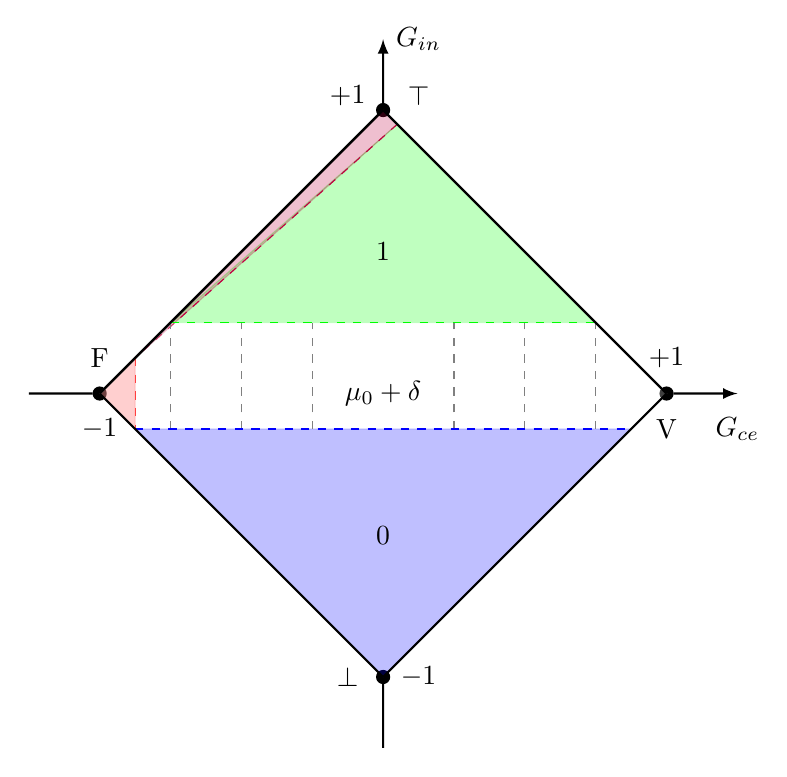
\begin{tikzpicture}[scale=0.90]
\tikzset{ >=latex, inner sep=0pt, outer sep=0pt,  }

%\draw [lightgray, dashed](0,0) grid (10,10);

\node [fill=black, circle] (V) at (9,5) {:};
\node [fill=black, circle] (F) at (1,5) {:};
\node [fill=black, circle] (T) at (5,9) {:};
\node [fill=black, circle] (L) at (5,1) {:};

\draw [->, thick] (V)   -- (10,5);
\draw [    thick] (0,5) -- (F);
\draw [->, thick] (T)   -- (5,10);
\draw [    thick] (5,0) -- (L);

\node at (10,4.5) {$G_{ce}$};
\node at (5.5,10) {$G_{in}$};

\node at (4.5,9.2) {$+1$};
\node at (9.0,5.5) {$+1$};
\node at (5.5,1.0) {$-1$};
\node at (1.0,4.5) {$-1$};

\node at (9.0,4.5) {V};
\node at (1.0,5.5) {F};
\node at (5.5,9.2) {$\top$};
\node at (4.5,1.0) {$\bot$};
%!@#

% liga-desliga
\draw [fill, green,nearly transparent] (5.2,8.8) -- (2.0,6.0) -- (8.0,6.0) -- (5.2,8.8);
\draw [fill,  blue,nearly transparent] (5.0,1.0) -- (8.5,4.5) -- (1.5,4.5) -- (5.0,1.0);
%\draw [white, thick] (1.0,5.0) -- (9.0,5.0);
\node at (5.0,7.0) {1};
\node at (5.0,3.0) {0};

% zona morta
\draw [fill, red,nearly transparent] (1.0,5.0) -- (1.5,5.5) -- (1.5,4.5) -- (1.0,5.0);
\draw [thick] (5.0,9.0) -- (1.0,5.0);
\draw [dashed, red] (1.5,5.5) -- (1.5,4.5);

% zona de travamento 
%\draw [fill, yellow, nearly transparent] (1.5,5.5) -- (5.0,9.0) -- (5.2,8.8) -- (1.5,5.5);
\draw [fill, purple, nearly transparent] (1.5,5.5) -- (5.0,9.0) -- (5.2,8.8) -- (1.5,5.5);
\draw [dashed, purple] (5.2,8.8) -- (1.5,5.5);
\draw [thick] (5.0,9.0) -- (1.0,5.0);


% zona de trabalho
\draw [fill, white,nearly transparent] (1.0,5.0) -- (2.0,6.0) -- (8.0,6.0) -- (9.0,5.0) -- (8.5,4.5)--(1.5,4.5) -- (1.0,5.0);
\draw [gray, dashed] (2.0,4.5) -- (2.0,6.0);
\draw [gray, dashed] (3.0,4.5) -- (3.0,6.0);
\draw [gray, dashed] (4.0,4.5) -- (4.0,6.0);
\draw [gray, dashed] (6.0,4.5) -- (6.0,6.0);
\draw [gray, dashed] (7.0,4.5) -- (7.0,6.0);
\draw [gray, dashed] (8.0,4.5) -- (8.0,6.0);
\draw [dashed, green] (2.0,6.0) -- (8.0,6.0);
\draw [dashed, blue] (1.5,4.5) -- (8.5,4.5);

\node at (5.0,5.0) {$\mu_0 + \delta$};

% Estados extremos
\draw [thick] (9,5) -- (5,9);
\draw [thick] (5,9) -- (1,5);
\draw [thick] (1,5) -- (5,1);
\draw [thick] (5,1) -- (9,5);

\end{tikzpicture}
\label{fig:diagramaPereiraLeao}

{\small Fonte: Próprio autor }
\end{figure}
%%%%%%%%%%%%%%%%%%%%%%%%%%%%%%%%%%%%%%%%%%%%%%%%%%

O diagrama mostra um controlador que possui algumas das regiões descritas anteriormente,
porém a região de verdade e a região de máxima inconsistência negativa tendendo a falsidade
não são implementados nesta primeira versão do controlador
pois assume-se que o sistema está ajustado para não apresentar saturação
e não produzir acionamento involuntário.

Cada região do diagrama produz um sinal no controlador de forma a
atender os requisitos de desempenho do sistema:
\begin{itemize}

\item Região de incerteza admitida:
Considerando a janela entre o $G_{in} < 0,10$ e $G_{in} > -0,05$
a região em que o controlador irá atuar ativamente,
fora do corte, na variável manipulada do sistema controlado,
aplicando o valor desejado somado a um fator de correção para dirimir o erro;

\item Região de incerteza positiva:
A região $G_{in} \ge 0,1$ gera na saída o seu valor máximo, $1,0$.
Desta forma o sistema controlado recebe sinal máximo de
acionamento, gerando a resposta mais rápida possível até que alcance
um grau de incerteza menor do que 0,1, correspondente a um erro
menor do que $10\%$.

\item Região de incerteza negativa:
Na região com $Gin \le -0,05$ a saída assume o valor nulo, $0,0$.
Assim quando o sistema controlado estiver com
uma velocidade acima do desejado, acima de $5\%$,o desligamento
controlado da saída possibilita a redução mais rápida possível na
velocidade controlada, considerando que não há uma alimentação
reversa para atuar ativamente na redução da velocidade.

\item Região de falsidade:
Corresponde a região de não linearidade correspondente a zona morta,
para valores com limiar do $G_{ce} < 0,1$,
região em que o sistema não responde a um acionamento de baixa velocidade.

\item Região de máxima inconsistência positiva tendendo a falsidade:
Essa região no controlador deve possuir um atraso para evitar alerta inadequado
no momento inicial de uma partida do sistema,
mas que passados os momentos iniciais,
qualquer momento em que o ponto de operação esteja sobre essa região,
produz um sinal nulo na saída para evitar sobrecarga pelo possível travamento
ou abertura do acoplamento com o sensor,
bem como um alerta ao operador.

\end{itemize}



 






\newpage



































%\section{ A região de operação }

%Para a região de operação, 
%foi estipulado um valor de grau de incerteza
%para atender os requisitos de desempenho do sistema,
%podendo ser alterado posteriormente após testes empíricos.
%O grau de incerteza está definido entre o intervalo menor do que 0,1 ($Gin < 1$) 
%e maior do que -0,05 ($Gin > -0,05$). Assumindo um valor inicial para
%a variável manipulada equivalente a um controle em malha aberta, sendo
%assim a resposta do controlador é o próprio $\mu_0$ como mostra a
%Figura \ref{fig:regiaoAtiva}.





%%%%%%%%%%%%%%%%%%%%%%%%%%%%%%%%%%%%%%%%%%%%%%% Fg
%\begin{figure}[!h]%%%%%%%%%%%%%%%%%%%%%%%%%%%%%%%%
%\centering
%\caption{Representação da região ativa no reticulado da LPA$E\tau$}
%\begin{tikzpicture}[scale=0.80]
%\tikzset{ >=latex, inner sep=0pt, outer sep=0pt,  }

%\draw [lightgray, dashed](0,0) grid (10,10);

%\node [fill=black, circle] (V) at (9,5) {:};
%\node [fill=black, circle] (F) at (1,5) {:};
%\node [fill=black, circle] (T) at (5,9) {:};
%\node [fill=black, circle] (L) at (5,1) {:};

%\draw [->, thick] (V)   -- (10,5);
%\draw [    thick] (0,5) -- (F);
%\draw [->, thick] (T)   -- (5,10);
%\draw [    thick] (5,0) -- (L);

%\draw [thick] (V) -- (T);
%\draw [thick] (T) -- (F);
%\draw [thick] (F) -- (L);
%\draw [thick] (L) -- (V);

%\node at (10,4.5) {$G_{ce}$};
%\node at (5.5,10) {$G_{in}$};

%\node at (4.5,9.2) {$+1$};
%\node at (9.0,5.5) {$+1$};
%\node at (5.5,1.0) {$-1$};
%\node at (1.0,4.5) {$-1$};

%\node at (9.0,4.5) {V};
%\node at (1.0,5.5) {F};
%\node at (5.5,9.2) {$\top$};
%\node at (4.5,1.0) {$\bot$};

%\draw [fill, red,nearly transparent] (1.0,5.0) -- (1.5,5.5) -- (1.5,4.5) -- (1.0,5.0);
%\draw [fill, purple, nearly transparent] (1.5,5.5) -- (5.0,9.0) -- (5.2,8.8) -- (1.5,5.5);
%\draw [fill, blue, nearly transparent] (5.0,1.0) -- (8.5,4.5) -- (1.5,4.5) -- (5.0,1.0);
%\draw [fill, green, nearly transparent] (5.2,8.8) -- (2.1,6.0) -- (8.0,6.0) -- (5.2,8.8);

%\draw [thick] (5.0,9.0) -- (1.0,5.0);

%\node at (5.0,7.0) {1};
%\node at (5.0,5.0) {$\mu_0$};
%\node at (5.0,3.0) {0};

%\end{tikzpicture}
%\label{fig:regiaoAtiva}

%{\small Fonte: Próprio autor }
%\end{figure}
%%%%%%%%%%%%%%%%%%%%%%%%%%%%%%%%%%%%%%%%%%%%%%%%%%









 
%%% Cap Resultados
%Aplicando um degrau à entrada do sistema, 
%podemos perceber o gráfico da 
%Figura \ref{fig:acaoLPAEtgct100} 
%que o tempo de acomodação é reduzido drasticamente, 
%apesar do sobressinal gerado, 
%este não apresenta problema por estar 
%dentro da tolerância aceitável. 



%%%%%%%%%%%%%%%%%%%%%%%%%%%%%%%%%%%%%%%%%%%%%% Img
%\begin{figure}[!htb]%%%%%%%%%%%%%%%%%%%%%%%%%%%%%%
%\caption{Ação de controle utilizando LPA$E\tau$}
%\vspace{-1cm}\center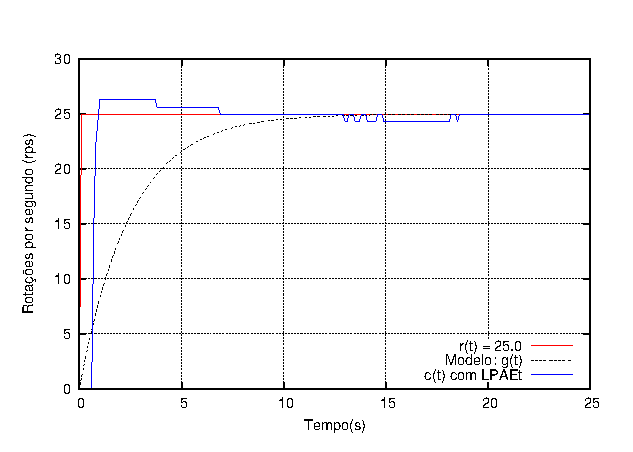
\includegraphics[scale=1.6]{./imagens/LPAEt-gct100.eps}
%\label{fig:acaoLPAEtgct100}

%{\small Fonte: Próprio autor}
%\end{figure}
%%%%%%%%%%%%%%%%%%%%%%%%%%%%%%%%%%%%%%%%%%%%%%%%%%





%######################################
%\begin{comment}


%\begin{figure}[!h]
%\centering
%\caption{Representação da região ativa no reticulado da LPA$E\tau$}
%\begin{tikzpicture}[scale=0.80]
%\tikzset{ >=latex, inner sep=0pt, outer sep=0pt,  }

%%\draw [lightgray, dashed](0,0) grid (10,10);

%\node [fill=black, circle] (V) at (9,5) {:};
%\node [fill=black, circle] (F) at (1,5) {:};
%\node [fill=black, circle] (T) at (5,9) {:};
%\node [fill=black, circle] (L) at (5,1) {:};

%\draw [->, thick] (V)   -- (10,5);
%\draw [    thick] (0,5) -- (F);
%\draw [->, thick] (T)   -- (5,10);
%\draw [    thick] (5,0) -- (L);

%\draw [thick] (V) -- (T);
%\draw [thick] (T) -- (F);
%\draw [thick] (F) -- (L);
%\draw [thick] (L) -- (V);

%\draw[thick] (SW) rectangle (NE);
%\fill[nearly transparent] (SW) rectangle (NE);

%\node at (10,4.5) {$G_{ce}$};
%\node at (5.5,10) {$G_{in}$};

%\node at (4.5,9.2) {$+1$};
%\node at (9.0,5.5) {$+1$};
%\node at (5.5,1.0) {$-1$};
%\node at (1.0,4.5) {$-1$};

%\node at (9.0,4.5) {V};
%\node at (1.0,5.5) {F};
%\node at (5.5,9.2) {$\top$};
%\node at (4.5,1.0) {$\bot$};

%\draw [fill, red,nearly transparent] (1.0,5.0) -- (1.5,5.5) -- (1.5,4.5) -- (1.0,5.0);
%\draw [fill, purple, nearly transparent] (1.5,5.5) -- (5.0,9.0) -- (5.2,8.8) -- (1.5,5.5);
%\draw [fill, blue, nearly transparent] (5.0,1.0) -- (8.0,4.0) -- (2.0,4.0) -- (5.0,1.0);
%\draw [fill, green, nearly transparent] (5.2,8.8) -- (2.1,6.0) -- (8.0,6.0) -- (5.2,8.8);

%\draw [fill, gray, nearly transparent] (4.0,6.0) -- (4.0,4.0)-- (6.0,4.0) -- (6.0,6.0) -- (4.0,6.0);


%\draw [dashed, purple] (5.2,8.8) -- (1.5,5.5);
%\draw [thick] (5.0,9.0) -- (1.0,5.0);
%\draw [gray,thick] (V) -- (F);


%\node at (5.0,7.0) {1};
%\node at (3.0,5.0) {$\mu_0 + \delta_0$};
%\node at (5.0,5.0) {$\mu_0 + \delta_1$};
%\node at (7.0,5.0) {$\mu_0 + \delta_n$};
%\node at (5.0,3.0) {0};

%\end{tikzpicture}
%\label{fig:regiaoAtivaMuDeltaN}

%{\small Fonte: Próprio autor }
%\end{figure}


%\end{comment}
%######################################




%Caso o tempo de 1 segundo seja muito alto para um 
%determinado processo, 
%para as perturbações envolvidas no processo,
%o tempo pode ser alterado para gerar uma resposta 
%mais rápida ou mais lenta. 




%%%%%%%%%%%%%%%%%%%%%%%%%%%%%%%%%%%%%%%%%%%%%%%%%%%%%%%%%%%%
%%%%%%%%%%%%%%%%%%%%%%%%%%%%%%%%%%%%%%%%%%%%%%%%%%%%%%%%%%%%


%\section{Diagrama PEREIRA-LEÃO}

%A LPA$E\tau$ pode estabelecer uma relação de semelhança com parâmetros
%típicos em automação e controle,
%de modo que podem ser facilmente interpretados e correlacionadas com
%variáveis manipulada e controlada, valores desejados e de sensores,
%bem como não linearidades, zona morta, saturação e histerese.



%%%%%%%%%%%%%%%%%%%%%%%%%%%%%%%%%%%%%%%%%%%%%% Fig
%\begin{figure}[!h]%%%%%%%%%%%%%%%%%%%%%%%%%%%%%%%%
%\centering
%\caption{Representação da LPA$E\tau$ no Diagrama Pereira-Leão}
%\begin{tikzpicture}[scale=0.70]
%\tikzset{ >=latex, inner sep=0pt, outer sep=0pt,  }

%\draw [lightgray, dashed](0,0) grid (10,10);

%\node [fill=black, circle] (V) at (9,5) {:};
%\node [fill=black, circle] (F) at (1,5) {:};
%\node [fill=black, circle] (T) at (5,9) {:};
%\node [fill=black, circle] (L) at (5,1) {:};

%\draw [->, thick] (V)   -- (10,5);
%\draw [    thick] (0,5) -- (F);
%\draw [->, thick] (T)   -- (5,10);
%\draw [    thick] (5,0) -- (L);

%\draw [thick] (V) -- (T);
%\draw [thick] (T) -- (F);
%\draw [thick] (F) -- (L);
%\draw [thick] (L) -- (V);

%\node at (10,4.5) {$G_{c}$};
%\node at (5.5,10) {$G_{i}$};

%\node at (4.5,9.2) {$+1$};
%\node at (9.0,5.5) {$+1$};
%\node at (5.5,1.0) {$-1$};
%\node at (1.0,4.5) {$-1$};

%\node at (9.0,4.5) {V};
%\node at (1.0,5.5) {F};
%\node at (5.5,9.2) {$\top$};
%\node at (4.5,1.0) {$\bot$};


%\draw [fill, purple,nearly transparent] (9.0,5.0) -- (8.5,5.5) -- (8.5,4.5) -- (9.0,5.0);
%\node at (10.0,7.5) {Região de};
%\node at (10.0,6.5) {Verdade};
%\draw [->, thick] (9.5,6.0) -- (8.70,5.20);

%\draw [fill, red,nearly transparent] (1.0,5.0) -- (1.5,5.5) -- (1.5,4.5) -- (1.0,5.0);
%\node at (0.0,3.5) {Região de};
%\node at (0.0,2.5) {Falsidade};
%\draw [->, thick] (0.5,4.0) -- (1.30,4.80);

%\draw [fill, green,nearly transparent] (1.5,5.5)--(2,6)--(8,6)--(8.5,5.5)--(8.5,4.5)--(8,4)--(2,4)--(1.5,4.5) -- (1.5,5.5);
%\node at (5.0,5.5) {Região de};
%\node at (5.0,4.5) {Trivialidade Admitida};



%\node at (0.0,9.5) {Região de Incerteza};
%\node at (0.0,8.5) {Máxima Positiva};
%\draw [->, thick] (2.5,8.0) -- (4.0,7.50);

%\node at (10.0,2.5) {Região de};
%\node at (10.0,1.5) {Incerteza Máxima Negativa};
%\draw [->, thick] (8.0,2.5) -- (6.00,3.00);

%\draw [fill, purple, nearly transparent] (1.5,5.5) -- (5.0,9.0) -- (5.2,8.8) -- (1.5,5.5);
%\draw [fill, blue, nearly transparent] (5.0,1.0) -- (8.5,4.5) -- (1.5,4.5) -- (5.0,1.0);
%\draw [fill, green, nearly transparent] (5.2,8.8) -- (2.1,6.0) -- (8.0,6.0) -- (5.2,8.8);

%\draw [thick] (5.0,9.0) -- (1.0,5.0);

%\node at (5.0,7.0) {1};
%\node at (5.0,5.0) {$\mu_0 + \delta$};
%\node at (5.0,3.0) {0};

%\draw [dashed, gray] (2.5,6.0) -- (2.5,4.5);
%\draw [dashed, gray] (3.5,6.0) -- (3.5,4.5);
%\draw [dashed, gray] (6.5,6.0) -- (6.5,4.5);
%\draw [dashed, gray] (7.5,6.0) -- (7.5,4.5);
%\draw [dashed, lightgray] (4.5,6.0) -- (4.5,4.5);
%\draw [dashed, lightgray] (5.5,6.0) -- (5.5,4.5);

%\end{tikzpicture}
%\label{fig:diagramaPereiraLeao}

%{\small Fonte: Próprio autor }
%\end{figure}
%%%%%%%%%%%%%%%%%%%%%%%%%%%%%%%%%%%%%%%%%%%%%%%%%%




%A aplicação da LPA$E\tau$ conforme estudada e implementada neste trabalho requer como
%proposição a correspondência direta à variável manipulada em seu valor máximo.
%Este valor máximo deve corresponder a condição verdade do diagrama.
%Assim, a proposição é verdadeira quando o máximo da variável manipulada é alcançada.

%Toda proposição apresenta duas anotações,
%sendo o grau de evidência favorável correspondente ao valor de referência do sistema, ou seja,
%ao valor desejado, $\mu$, enquanto que o grau de evidência contrária corresponde ao
%complemento do sinal do sensor, $\lambda$, desta forma,
%quando o sensor apresenta valor máximo, $\lambda = 0$, de maneira oposta,
%quando o sensor apresenta valor mínimo, $\lambda = 1$.

%O ponto gerado pela combinação $(\mu,\lambda)$ ao estar contido respectivamente em $(0,1)$,
%corresponde ao mínimo da variável controlada,
%enquanto que para a combinação extrema $(1,0)$ corresponde ao máximo da variável controlada.

%A primeira etapa de implementação do controlador utilizando LPA$E\tau$
%conforme apresentada neste trabalho,
%deve-se setar o máximo da variável manipulada com o máximo valor apresentado pelo sensor,
%de forma análoga a uma sistema em malha aberta, em que o máximo da referência produz o máximo
%valor da variável controlada.

%Para a condição em que o valor desejado e o sensor apresentam igualdade,
%o Grau de Incerteza é nulo, e o sistema não apresenta erro. Isso ocorre sempre que a
%anotação produzir um ponto sobre a reta do Grau de Certeza. Para uma variação dentro
%dos parâmetros admissíveis, a região correspondente, situada no entorno da linha de Grau de Certeza,
%próximo ao zero tanto quanto o sistema admitir, 
%recebe o nome de Região de Trivialidade Admitida. 


%A região que apresenta um Grau de Incerteza elevado recebe o nome de
%Região de Incerteza Máxima Positiva,
%e para o sistema estudado corresponde a condição em que a variável controlada está muito abaixo
%do valor desejado, assim, elevando a variável manipulada ao seu valor máximo, afim de anular o erro.

%A região que apresenta o Grau de de Incerteza mais baixo, recebe o nome de
%Região de Incerteza Máxima Negativa,
%o que corresponde à condição em que a variável controlada apresenta valor bem acima do valor desejado,
%produzindo um valor nulo na variável manipulada, situação tida como adequada para a situação aqui
%vista, e deve ser avaliada para cada situação em que o controlador venha ser utilizado.

%O conceito de zona morta pode ser representado pela região de falsidade,
%pois localiza-se em uma região em que a variável desejada apresenta um valor em que o sistema físico
%não reage ao estímulo, tendo um limiar em que a inércia de partida é vencida e o
%sistema se coloca em movimento, no caso do motor acoplado a uma carga.

%Em automação e controle, a zona morta é um conceito bem comum, assim como a saturação,
%que no diagrama Pereira-Leão pode ser apresentada na região de verdade, porém,
%ao ajustar os parâmetros,
%para o máximo da variável manipulada equivalente a máxima resposta do sistema,
%a saturação não ocorre, ou fica restrita a condição de verdade.




%A condição de falsidade é o Valor mínimo da variável controlada;
%O Grau de evidência favorável( $\mu$ ) como valor desejado, ou setpoint;
%O grau de evidência desfavorável ( $\lambda$ ) como valor do sensor da variável controlada;
%A região de falsidade é caracterizada como zona morta;
%A região de verdade é caracterizada como saturação;
%A trivialidade(incerteza) admitida corresponde a histerese.






%%%%%%%%%%%%%%%%%%%%%%%%%%%%%%%%%%%%%%%%%%%%%% Fig
%\begin{figure}[!h]%%%%%%%%%%%%%%%%%%%%%%%%%%%%%%%%
%\centering
%\caption{Representação da LPA$E\tau$ no Diagrama Pereira-Leão}
%\begin{tikzpicture}[scale=0.70]
%\tikzset{ >=latex, inner sep=0pt, outer sep=0pt,  }

%\draw [lightgray, dashed](0,0) grid (10,10);

%\node [fill=black, circle] (V) at (9,5) {:};
%\node [fill=black, circle] (F) at (1,5) {:};
%\node [fill=black, circle] (T) at (5,9) {:};
%\node [fill=black, circle] (L) at (5,1) {:};

%\draw [->, thick] (V)   -- (10,5);
%\draw [    thick] (0,5) -- (F);
%\draw [->, thick] (T)   -- (5,10);
%\draw [    thick] (5,0) -- (L);

%\draw [thick] (V) -- (T);
%\draw [thick] (T) -- (F);
%\draw [thick] (F) -- (L);
%\draw [thick] (L) -- (V);

%\node at (10,4.5) {$G_{c}$};
%\node at (5.5,10) {$G_{ct}$};

%\node at (4.5,9.2) {$+1$};
%\node at (9.0,5.5) {$+1$};
%\node at (5.5,1.0) {$-1$};
%\node at (1.0,4.5) {$-1$};

%\node at (9.0,4.5) {V};
%\node at (1.0,5.5) {F};
%\node at (5.5,9.2) {$\top$};
%\node at (4.5,1.0) {$\bot$};

%\draw [fill, red,nearly transparent] (1.0,5.0) -- (1.5,5.5) -- (1.5,4.5) -- (1.0,5.0);
%\draw [fill, purple, nearly transparent] (1.5,5.5) -- (5.0,9.0) -- (5.2,8.8) -- (1.5,5.5);
%\draw [fill, blue, nearly transparent] (5.0,1.0) -- (8.5,4.5) -- (1.5,4.5) -- (5.0,1.0);
%\draw [fill, green, nearly transparent] (5.2,8.8) -- (2.1,6.0) -- (8.0,6.0) -- (5.2,8.8);

%\draw [thick] (5.0,9.0) -- (1.0,5.0);

%\node at (5.0,7.0) {1};
%\node at (5.0,5.0) {$\mu_0 + \delta$};
%\node at (5.0,3.0) {0};

%\draw [dashed, gray] (2.5,6.0) -- (2.5,4.5);
%\draw [dashed, gray] (3.5,6.0) -- (3.5,4.5);
%\draw [dashed, gray] (6.5,6.0) -- (6.5,4.5);
%\draw [dashed, gray] (7.5,6.0) -- (7.5,4.5);
%\draw [dashed, lightgray] (4.5,6.0) -- (4.5,4.5);
%\draw [dashed, lightgray] (5.5,6.0) -- (5.5,4.5);

%\end{tikzpicture}
%\label{fig:diagramaPereiraLeao}

%{\small Fonte: Próprio autor }
%\end{figure}
%%%%%%%%%%%%%%%%%%%%%%%%%%%%%%%%%%%%%%%%%%%%%%%%%%


